\documentclass[notitlepage, a4paper]{article}

%\usepackage[left=1cm,right=1cm,top=1.5cm,bottom=1.5cm,
%            headheight=14.92502pt]{geometry}

%\usepackage{fancyhdr}
%\pagestyle{fancy}
%\fancyhead[LE,RO]{\today}
%\fancyhead[LO,RE]{Albert \v{S}ilvans S3400166}
%%\fancyhead[CE]{Circle Map derivation}
%\fancyhead[C]{MSc Thesis}
%\fancyfoot{}
%\fancyfoot[C]{}
%\fancyfoot[RO, LE] {\thepage}

\title{Complex Dynamics of Magnetic Billiards in a Torus}
\author{Albert \v{S}ilvans, s3400166}

\usepackage{amsthm}
\usepackage{amsmath}
\usepackage{amsfonts}
\usepackage{amssymb}
\usepackage{dsfont}
\renewcommand{\qedsymbol}{$\blacksquare$}

\theoremstyle{definition}
\newtheorem{exercise}{Exercise}
\newtheorem{proposition}{Proposition}
\newtheorem{definition}{Definition}
\newtheorem{theorem}{Theorem}
\newtheorem{lemma}{Lemma}

\usepackage{eucal}
%\usepackage{rsfso}
\usepackage{mathrsfs}
\usepackage{enumitem}
\usepackage{cleveref}
\usepackage{subcaption}
\usepackage{booktabs}
\usepackage{array}
\usepackage{url}
\usepackage{multirow}

\newcommand{\D}{\text{d}}
\newcommand{\sech}{\text{sech}}
\newcommand{\csch}{\text{csch}}
\newcommand{\arsinh}{\text{arsinh}}
\newcommand{\sgn}[1]{\text{sgn}(#1)}
\newcommand{\Span}{\text{span}}
\newcommand{\ran}{\text{ran}}
\def\one{\rlap{\mbox{\small\rm 1}}\kern.15em 1}
\def\ind#1{\1_{#1}}
\newcommand{\Sout}{S_\text{out}}
\newcommand{\Sin}{S_\text{in}}

\usepackage{csquotes}

\usepackage{xcolor}
\usepackage{soul}

\usepackage{graphicx}
\graphicspath{{./code_and_figures/}}

\usepackage{listings}

\definecolor{codegreen}{rgb}{0,0.6,0}
\definecolor{codegray}{rgb}{0.5,0.5,0.5}
\definecolor{codepurple}{rgb}{0.58,0,0.82}
\definecolor{backcolour}{rgb}{0.95,0.95,0.92}

\lstdefinestyle{mystyle}{
    backgroundcolor=\color{backcolour},   
    commentstyle=\color{codegreen},
    keywordstyle=\color{magenta},
    numberstyle=\tiny\color{codegray},
    stringstyle=\color{codepurple},
    basicstyle=\ttfamily\footnotesize,
    breakatwhitespace=false,         
    breaklines=true,                 
    captionpos=b,                    
    keepspaces=true,                 
    numbers=left,                    
    numbersep=5pt,                  
    showspaces=false,                
    showstringspaces=false,
    showtabs=false,                  
    tabsize=2
}

\lstset{style=mystyle}

\usepackage{tikz}

\begin{document}

\maketitle
\newpage
\tableofcontents
\listoffigures
\newpage

\section{Introduction}


Mathematical billiards is a broad topic in dynamical systems which studies the long term motion of a particle in the presence of an obstruction. The obstruction can be a boundary upon which the particle collides and then is elastically reflected, or there can be a vector field that deflects the particle, for example, a magnetic field. In this paper we consider the latter. We take the work \cite{Knauf_2017} and \cite{Gasiorek_2021} as inspiration.

Let $H:\mathbb R^3\times\mathbb R^3\to\mathbb R$ be a magnetic Hamiltonian function:
\begin{align}\label{eq:magnetichamiltonian}
H(q,p) &= \frac{1}{2}\left\|p - A(q)\right\|^2
\end{align}
where $q=(q_1,q_2,q_3)$ is position, $p=(p_1,p_2,p_3)$ is momentum, $A:\mathbb R^3\to\mathbb R^3$ is a magnetic vector field defined as follows:
\begin{align}
A(q) &= (-b(q_2 \mod 1),0,0)\one_S(q\!\mod 1) \\
S &= \{x\in \mathbb R^2 : \|x-1/2\|\le R\},
\end{align}
with magnetic field strength $b\in(0,\infty)$, and $R\in(0,1/2)$, the radius of the disk $S$ centered at $(1/2,1/2)$ in the plane. Lastly, $\one_S$ is an indicator function on $S$, that is $\one_S(x)=1$ if $x\in S$ and $\one_S(x)=0$ otherwise.

We note that $A$ is independent of $q_3$, so for $q_3=p_3=0$, a solution of the Hamiltonian equations of $H$ is contained within the $q_1q_2$-plane. So, we ignore the $q_3$ variable completely. Furthermore, $A$ is 1-periodic in both $q_1$ and $q_2$, so we can consider $H$ on the torus $\mathbb T =\mathbb R^2/\mathbb Z^2$ via the quotient. We will refer to $H$ on either surfaces interchangeably. Likewise, the periodicity of $A$ gives rise to a lattice of disks centered at the points $N+1/2$ for $N\in\mathbb Z^2$, we use the variable $S$ to refer to either the disc in $[0,1]^2$ or to the lattice, and make it clear which we are referring to when necessary.

The motion of a particle under $H$ in the interior and the exterior of $S$ is well understood. In the exterior of $S$ there is no magnetic field, so the particle experiences free motion and travels in a straight line. In the interior of $S$, we know that the particle travels along arcs of a \textit{Larmor} circle with \textit{Larmor} radius $\|p\|/b$. Since \cref{eq:magnetichamiltonian} is discontinuous along the boundary $\partial S$, we have an issue when considering particles that enter $\partial S$ tangentially, in which case the solution is not necessarily unique. In such cases, we assume the particle is in free motion. 

We see an example trajectory in \cref{fig:sensitive_trajectory} which demonstrates the types of motion exhibited by the system. In blue we indicate free motion, and in red we have motion in the magnetic field. The red segments should instead be circular arcs, we reserve some artistic liberty in this choice. We also only draw the boundary of disks that are hit by the particle, and skip the rest to improve legibility. Focusing now on the trajectory itself we see:
\begin{itemize}
\item erratic behavior, that is, the trajectory seems to bounce around in a chaotic manner;
\item evidence for quasi-periodic motion, specifically referring to the spot where the particle is trapped between four discs before eventually escaping;
\item two distinct scales, the intervals of magnetic motion serve as a perturbation or deflection and are rather local, while the intervals of free motion can be long and in fact can be arbitrarily long provided that the particle exits a disc at a shallow enough angle.
\end{itemize}
 
\begin{figure}[!th]
\centering
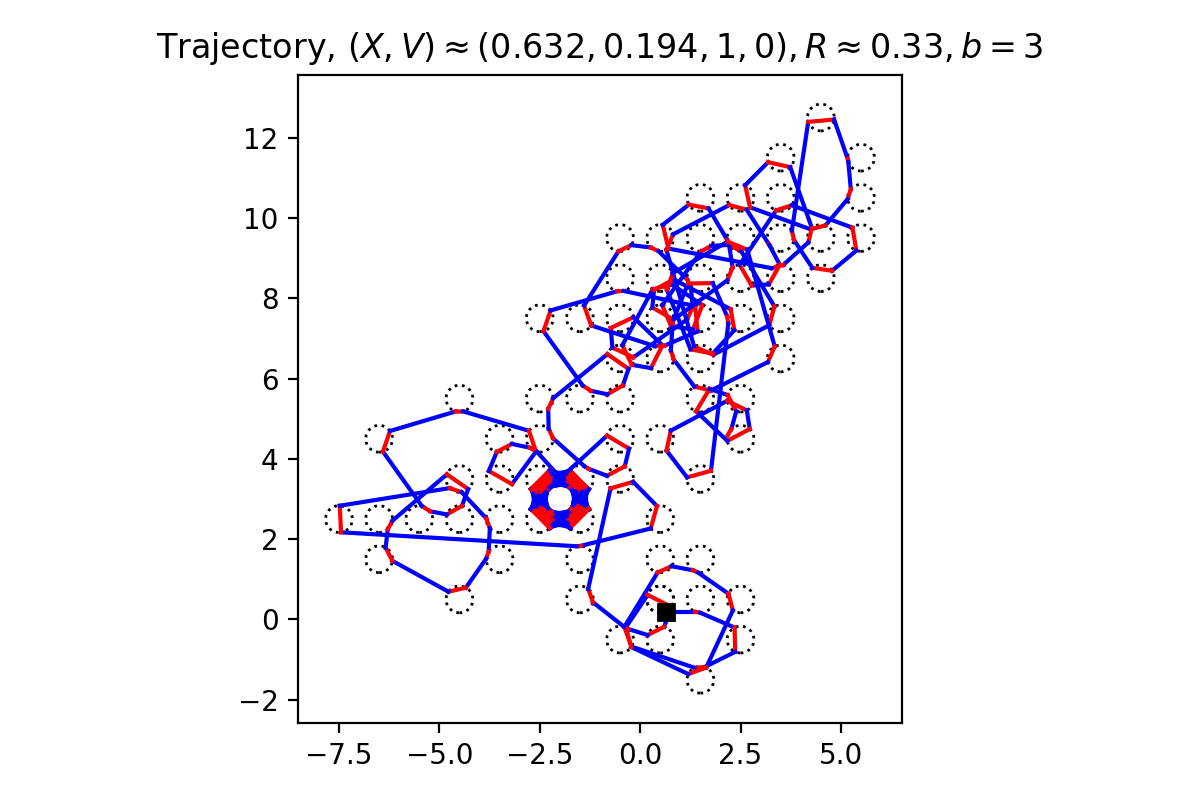
\includegraphics[width=\textwidth, trim={0 0cm 0 0cm}, clip]{sensitive_trajectory.png}
\caption{An example trajectory illustrating various types of motion.}
\label{fig:sensitive_trajectory}
\end{figure}
So far, we see that the motion is not trivial, and warrants study. What is not yet evident from \cref{fig:sensitive_trajectory} is the influence of the parameters $R$ and $b$ on the general behavior of the system. This is what we aim to better understand by the end of the paper. 


We outline how we study this system. We focus on varying $b$, and identify three modes for some $b_1,b_2\in\mathbb R$ with $b_1<b_2$. \hl{Continue this later.}



\begin{table}[!ht]
\centering
\renewcommand\arraystretch{2}
\begin{tabular}{>{\raggedright}p{0.2\linewidth}
				>{\raggedright}p{0.2\linewidth}
				>{\raggedright}p{0.2\linewidth}
				>{\raggedright\arraybackslash}p{0.2\linewidth}
                }
\toprule
 & $b<b_1$ & $b_1<b<b_2$ & $b_2<b$ \\
\midrule
Uniform perturbation in a disk 
  & \multirow{2}*{Usual } 
  & test cases (difficult in general)
  & Perturbation of Sinai Billiards (maybe) \\
Arbitrary perturbations
  & 
  & use paper by Donnay-Liverani
  & Hard?\\
\bottomrule
\end{tabular}
\caption{What it is that we want to do}
\label{tab:outline}
\end{table}






\newpage

\section{Weak magnetic fields and KAM theory}


We begin by recalling Kolmogorov-Arnold-Moser (KAM) theory, state one of the main KAM theorems, and briefly outline the main points of the theory before delving into its application. We refer the reader to \cite{Knauf_2018} and \cite{Seri_2022} for a more detailed account. We strongly recommend \cite{poschel82} for reference, as it is the version of KAM we use here. 


KAM theory is a method for studying perturbations of integrable Hamiltonian systems. Its origins lie in Celestial and Hamiltonian mechanics, where it was used to study the orbits of planets. Hamiltonian mechanics is a strong tool for modeling and studying systems, however it is strongest for conservative systems. Naturally, we find in practice many non-conservative systems, or conservative ones that are too complicated in full, in which case a smaller subsystem is modeled and the rest is viewed as a perturbation. We are interested in the second scenario, we denote by $H^0(q,p)$ an integrable Hamiltonian and by $H^1(q,p,\varepsilon)$ a perturbation. 

Focusing on the integrable case, it is known by the Liouville-Arnold theorem that there exist \textit{action-angle} coordinates so that $H^0:=H^0(p)$ can be expressed in terms of the action variable only. The equations of motion in action-angle coordinates are given by:
\begin{align*}
\dot q = \omega, \qquad \dot p = 0,
\end{align*}
where $\omega = \partial_pH^0(p)$ and $\partial_p H^0:I\to\Omega$ is the so-called \textit{frequency map}. In these action-angle coordinates, the phase space becomes $\mathbb T^n\times I$ where $I\subseteq\mathbb R^n$ and the dynamics of the system are completely expressed as rotations on the torus. Specifically, phase space is foliated into a family of invariant tori $\mathbb T^n\times\{p\}$ for each $p\in I\subseteq \mathbb R^n$. We consider only integrable Hamiltonians with a \textit{non-degenerate} frequency map, that is, $\det\partial_p^2 H^0\neq 0$. Now, KAM deals with Hamiltonians of the form
\begin{align*}
H(q,p) = H^0(p) + \varepsilon H^1(q,p),
\end{align*}
where $1\gg\varepsilon>0$ is considered small, $H^0$ is the integrable part and $H^1$ is the perturbation. We assume that $H$ is $2\pi$-periodic in each component of $q$. What KAM theory ensures is that under the correct conditions, a ``large'' subset $\Omega_{\gamma,\tau}\subseteq\Omega$, $\gamma,\tau>0$ of invariant tori of $H^0(p)$ are preserved, though possibly deformed, under the perturbation $H^1$. The set $\Omega_{\gamma,\tau}$ is given by:
\begin{align}\label{eq:smalldivisorcondition}
\Omega_{\gamma,\tau} = \left\{ \omega\in\Omega :
|\omega \cdot k| \ge \gamma|k|^{-\tau}, 0\neq k\in \mathbb Z^n \right\}.\\ \text{\color{red} make sure you understand the Cantor set construction on page 134\color{black}}
\end{align}
The condition for $\Omega_{\gamma,\tau}$ is called the \textit{small divisor condition}. It can be shown that for $\tau>n-1$ almost all points in $\mathbb R^n$ satisfy such a condition for the right choice of $\gamma$, so we can find such points in $\Omega$ as well. In the statement of the theorem we will see that $\gamma$ cannot be varied and must be fixed, since it comes in as a constant in the bound on the size of the perturbation, so we consider the \textit{Cantor} set 
\begin{align*}
\Omega_\gamma=\{\omega\in\Omega: d(\omega,\partial\Omega)\ge\gamma\}\cap\left(\bigcup_{\tau>n-1}\Omega_{\gamma,\tau}\right).
\end{align*}

We see $\Omega\backslash \bigcup_{\gamma>0}\Omega_\gamma$ is a set of measure zero, so the measure of $\Omega_\gamma$ becomes large for small $\gamma$ ,justifying the term ``large''. We can now give the KAM theorem as stated in \cite{poschel82}.

\begin{theorem}\label{thm:KAM}
Let the integrable Hamiltonian $H^0:\mathbb T^n\times I\to\mathbb R$ be real analytic and non-degenerate, such that the frequency map $\partial_p H^0:I\to\Omega$ is a diffeomorphism and let the perturbed Hamiltonian $H=H^0+\varepsilon H^1$ be of class $C^{\alpha\lambda+\lambda+\tau}$ with $\lambda>\tau+1>n$ and $\alpha>1$. Then there exists a positive $\gamma$-independent $\delta$ such that for $|\varepsilon|<\gamma^2\delta$ with $\gamma$ sufficiently small, there exists a diffeomorphism
\begin{align*}
\mathcal T: \mathbb T^n\times\Omega \to\mathbb T^n\times I,
\end{align*} 
which on $\mathbb T^n\times\Omega_\gamma$ transforms the equations of motion of $H$ into
\begin{align*}
\dot \theta=\omega,\qquad \dot\omega=0.
\end{align*}
The map $\mathcal T$ is of class $C^\alpha$ for non-integer $\alpha$ and close to the inverse of the frequency map; its Jacobian determinant is uniformly bounded from above and below.

In addition, if $H$ is of class $C^{\beta\lambda+\lambda+\tau}$ with $\alpha\le\beta\le\infty$, then one can modify $\mathcal T$ outside $\mathbb T^n\times\Omega_\gamma$ so that $\mathcal T$ is of class $C^\beta$ for noninteger $\beta$.
\end{theorem}

So, for $\omega\in\Omega_\gamma$, we can parametrize an invariant torus via the map $\theta\mapsto\mathcal T(\theta,\omega)$. There are a few theorems in use now that are titled the \textit{KAM theorem}, and they differ mainly whether they discuss analytic or smooth perturbations. It is easier to find sources discussing the analytic versions, since they provide stronger results about the invariant torii. Having said this, we use the $C^r$ version because it is easier to construct smooth approximations of discontinuous functions as opposed to analytically approximating them.

The Hamiltonian \eqref{eq:magnetichamiltonian2} we wish to study is discontinuous, which by itself is not suitable for the KAM theorem. We can, however, smoothly approximate the Hamiltonian by using \textit{mollifiers}. The \textit{standard mollifier} $\varphi:\mathbb R^n\to\mathbb R$ is the following function:
\begin{align*}
\varphi(x) = \left\{\begin{array}{ll}
c\exp\left(\frac{1}{|x|^2-1}\right), & |x| <1\\
0, & |x|\ge 1,
\end{array}
\right.
\end{align*}
where $c>0$ is a scaling factor chosen so that the integral of $\varphi$ over $\mathbb R^n$ is 1. Also, $\varphi$ is commonly called a \textit{bump} function, since its support is compact. For $\varepsilon>0$, let
\begin{align*}
\varphi_\varepsilon(x) = \frac{1}{\varepsilon^2}\varphi\left(\frac{x}{\varepsilon}\right),
\end{align*} 
this function has the following properties:
\begin{align*}
\varphi_\varepsilon\in C_c^\infty(\mathbb R^n),\quad
\varphi\ge 0,\quad
\int_{\mathbb R^n}\varphi =1,\quad
\text{supp}(\varphi_\varepsilon)\subset B_\varepsilon(0)=\{x\in\mathbb R^n:|x|<\varepsilon\},
\end{align*}
that is, the function $\varphi_\varepsilon$ is smooth in $\mathbb R^n$ with compact support, it is positive, its integral is 1, and the support of $\varphi_\varepsilon$ is fully contained in the unit ball of radius $\varepsilon>0$ centered at the origin.
  
Let $f\in L_{\text{loc}}^1(X)$ be a locally integrable function in $X \subseteq\mathbb R^n$. The \textit{mollification} of $f$ is defined as the convolution of $f$ with $\varphi_\varepsilon$, that is, $\varphi_\varepsilon*f:X_\varepsilon\to\mathbb R$ where $X_\varepsilon=\{x\in X: d(x,\partial X)>\varepsilon\}$. Explicitly,
\begin{align*}
f_\varepsilon(x) = \big(\varphi_\varepsilon * f\big)(x) = \int_X\varphi_\varepsilon(x-y)f(y)dy = \int_{B_\varepsilon(0)}\varphi_\varepsilon(y)f(x-y)dy,\quad x\in X_\varepsilon
\end{align*}

Some properties that the mollification $f_\varepsilon$ has are summarized here:
\begin{theorem}\label{thm:mollification}
Let $f\in L_{\text{loc}}^1(X)$. Then the mollification $f_\varepsilon$ has the following properties:
\begin{enumerate}
\item $f_\varepsilon\in C^\infty)(X_\varepsilon)$,
\item $f_\varepsilon\to f$ almost everywhere as $\varepsilon\to0$,
\item if $f$ is continuous on $X$, then $f_\varepsilon\to f$ as $\varepsilon\to0$ uniformly on compact subsebts of $X$,
\item if $1\le p <\infty$ and $f\in L_{\text{loc}}^p(X)$, then $f_\varepsilon\to f$ as $\varepsilon\to 0$ in $L_{\text{loc}}^p(X)$
\end{enumerate}
\end{theorem}
\begin{proof}
The proof of this theorem can be found in Appendix C of \cite{Evans_1998}
\end{proof}

What we gain from \Cref{thm:mollification} is not only a smooth approximation of our discontinuous Hamiltonian but an approximation that can be made arbitrarily precise almost everywhere. Of course, the points which cannot be approximated accurately are concentrated at the boundary of each disk, where the discontinuities lie. Despite this, it is reasonable to assume that for sufficiently small values of $\varepsilon$, the flow of the equations of motion provided by the mollified Hamiltonian approximate very well the flow of the disconitinuous one.
\subsection{Perturbations of linear motion}


\subsection{Perturbation of motion in a constant field}

\newpage

\section{Complexity and symbolic dynamics}
In this section we consider the dynamics of \eqref{eq:magnetichamiltonian} for $b\gg 0$, that is, in the case where KAM and perturbative methods are not readily applicable. We approach the system in an exploratory way: we look for (quasi)-periodic orbits, consider their stability, and see where stability is missing.

To this end, we prove the existence of a Poincar\'e section, later we induce ``coarse'' symbolic dynamics and apply the Lempel-Ziv complexity to make sense of the dynamics. What we find is rich dynamics and a visual method of analysis well suited for similar problems.

The phase space of our system is $\mathbb R^2\times\mathbb R^2$, however we can reduce the phase space to a Poincar\'e section as follows:
\begin{proposition}\label{prop:poincaresurface}
Let $S$ be the union of discs of radius $R$ centered at $\mathbb Z^2+1/2$. The sets $\Sin$ and $\Sout$ defined as:
\begin{align}
\label{def:poincaresectionIN}
\Sin &= \bigcup_{x\in\partial S} \{x\} \times \{v\in\mathbb R^2 : v\cdot (x-1/2) < 0\},\\
\label{def:poincaresectionOUT}
\Sout &= \bigcup_{x\in\partial S} \{x\} \times \{v\in\mathbb R^2 : v\cdot (x-1/2) > 0\},
\end{align}
are Poincar\'e sections for the system \eqref{eq:magnetichamiltonian}.
\end{proposition}
We prove this later. This helps visualize long term behavior, since the magnitude of the velocity of a trajectory is constant. Furthermore, we can pass the system to the torus, which reduces $S$ to one disc. So, when plotting we only need two dimensions: one to parametrize $\partial S$ and another for the velocity.

\subsection{First impressions and lots of quasiperiodicity}
%\subsection{First impressions and lots of quasiperiodicity}

For the remainder of this section we fix $R=1/3$ and $\|p\|=1$, we only vary $b$. In the figures below, we collect a few periodic and quasi-periodic orbits. For each figure, on the left is a plot of the trajectory in the plane, and on the right we give the trajectory restricted to the section $\Sout$. The depth of computation is 2000 entries into $\Sout$, unless stated otherwise. We discovered the trajectories in \cref{fig:penandpaperorbits} on paper, the rest were discovered using the methods we discuss later.

\begin{figure}[!th]
\centering
\begin{subfigure}{0.49\textwidth}
\centering
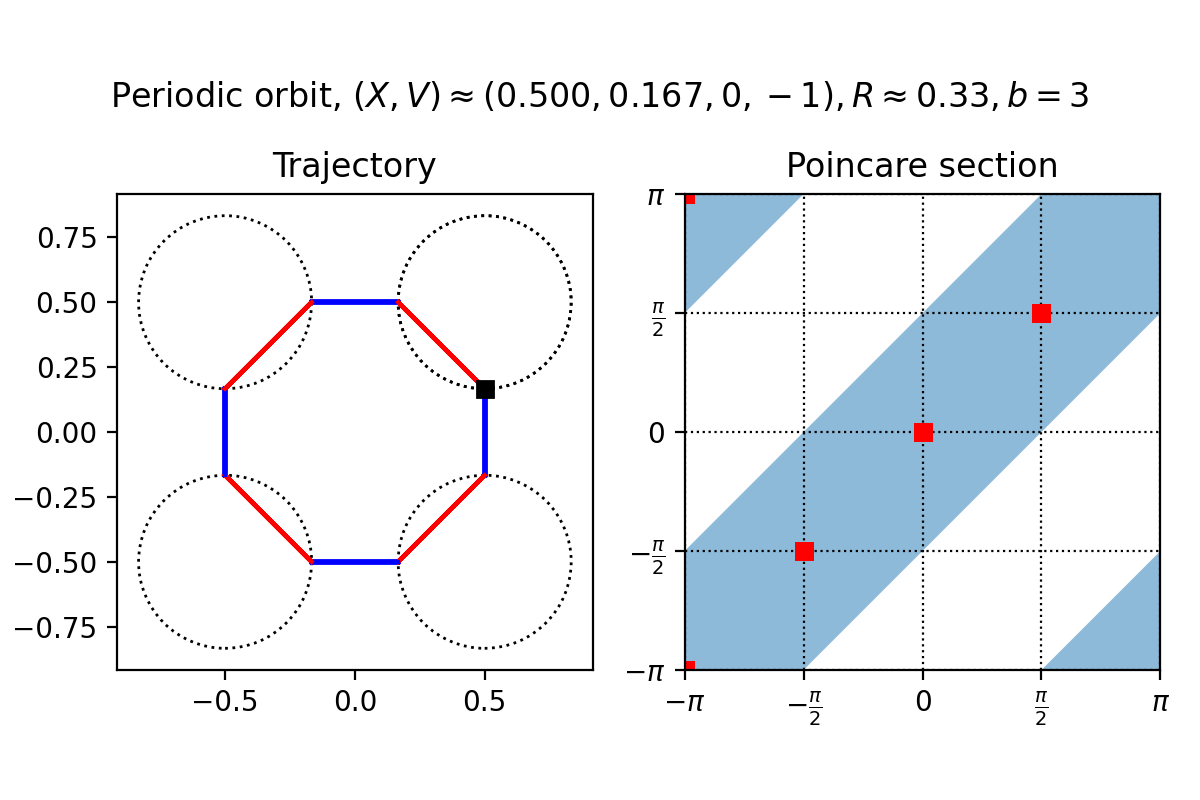
\includegraphics[width=\textwidth, trim={0 1cm 0 0cm}, clip]{stable_square_with_poincare.png}
\caption{}
\label{subfig:penandpaperorbits1}
\end{subfigure}
%
\begin{subfigure}{0.49\textwidth}
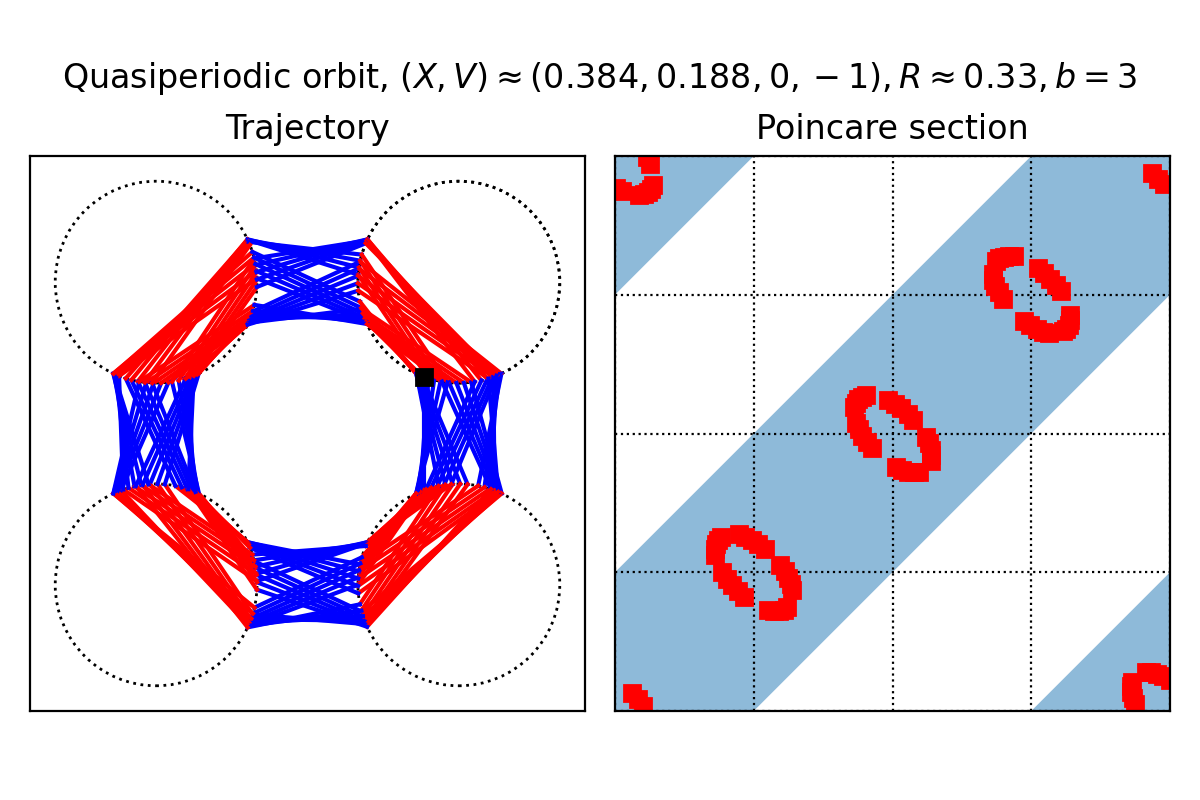
\includegraphics[width=\textwidth, trim={0 1cm 0 0cm}, clip]{perturbed_stable_square_with_poincare.png}
\caption{}
\label{subfig:penandpaperorbits2}
\end{subfigure}
\caption{Stable trajectories discovered analytically (more on next page).}
\end{figure}

\begin{figure}[!th]
\ContinuedFloat
\centering
\begin{subfigure}{0.49\textwidth}
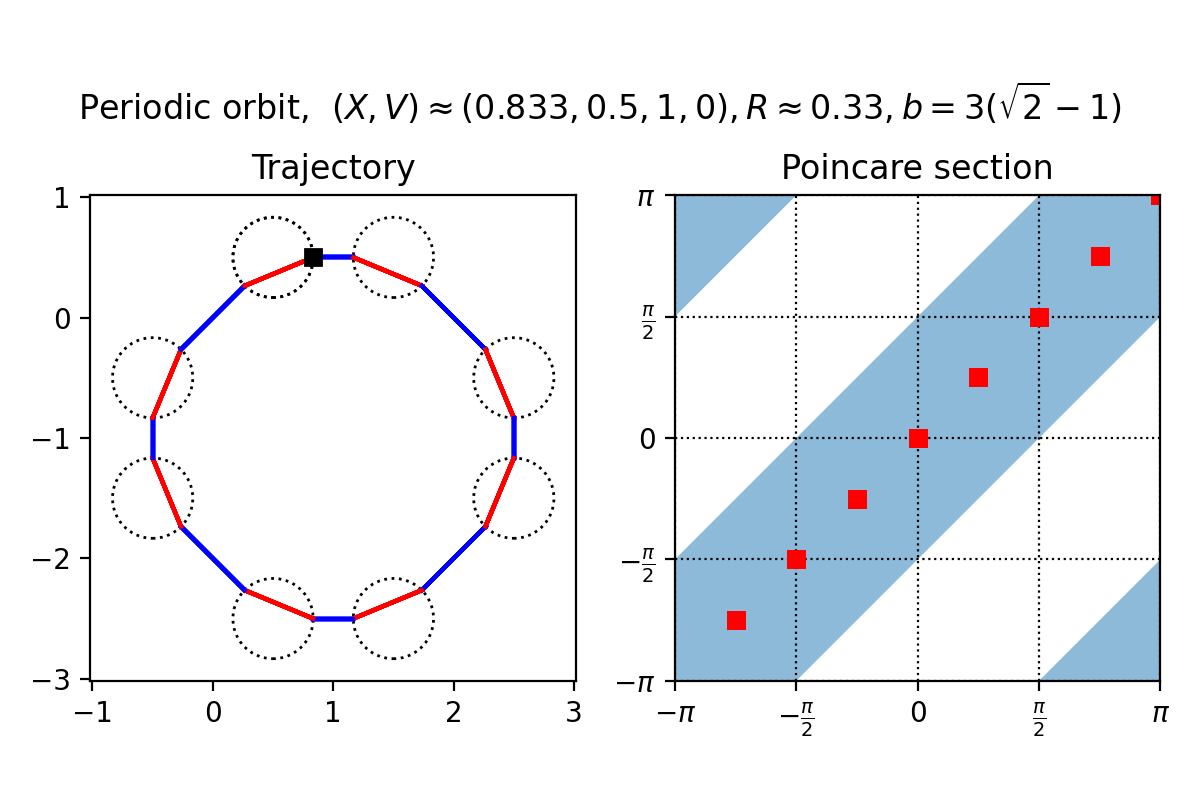
\includegraphics[width=\textwidth, trim={0 1cm 0 0cm}, clip]{stable_octagon_with_poincare.png}
\caption{}
\label{subfig:penandpaperorbits3}
\end{subfigure}
%
\begin{subfigure}{0.49\textwidth}
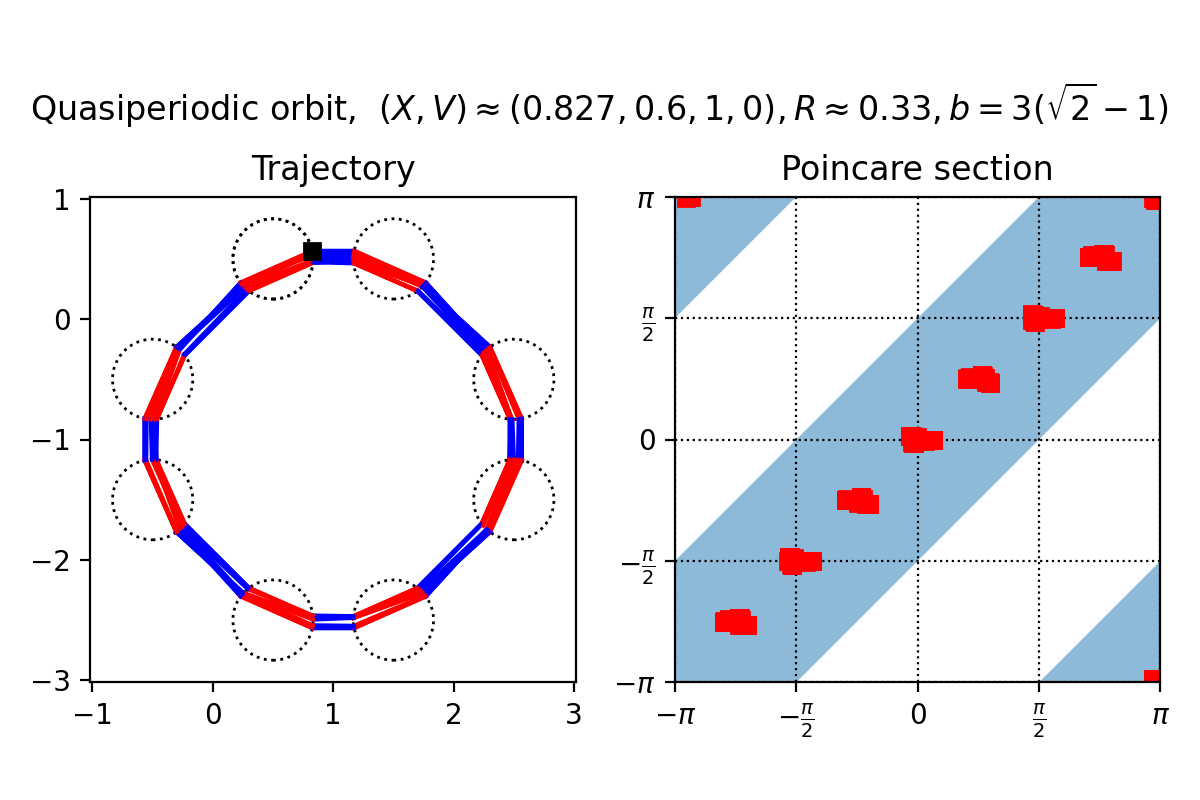
\includegraphics[width=\textwidth, trim={0 1cm 0 0cm}, clip]{perturbed_stable_octagon_with_poincare.png}
\caption{}
\label{subfig:penandpaperorbits4}
\end{subfigure}
%
\begin{subfigure}{0.49\textwidth}
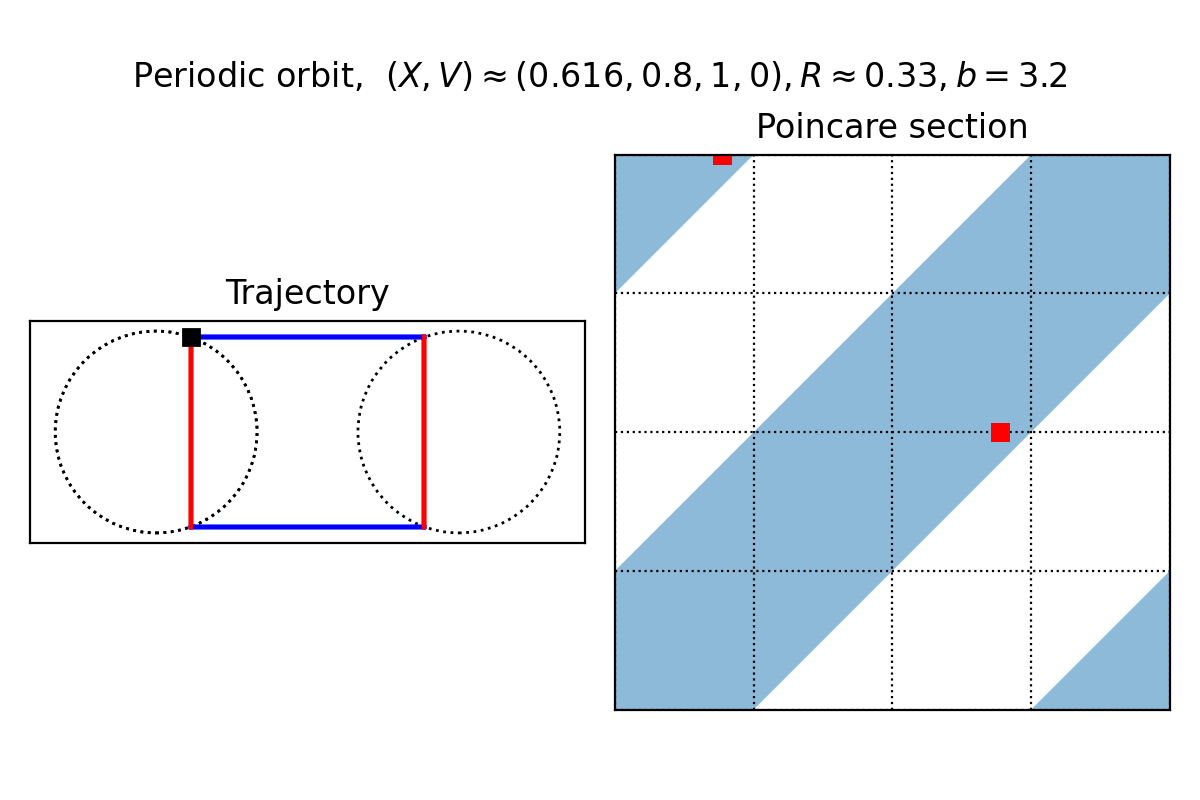
\includegraphics[width=\textwidth, trim={0 1cm 0 0cm}, clip]{unstable_square_with_poincare.png}
\caption{}
\label{subfig:penandpaperorbits5}
\end{subfigure}
%
\begin{subfigure}{0.49\textwidth}
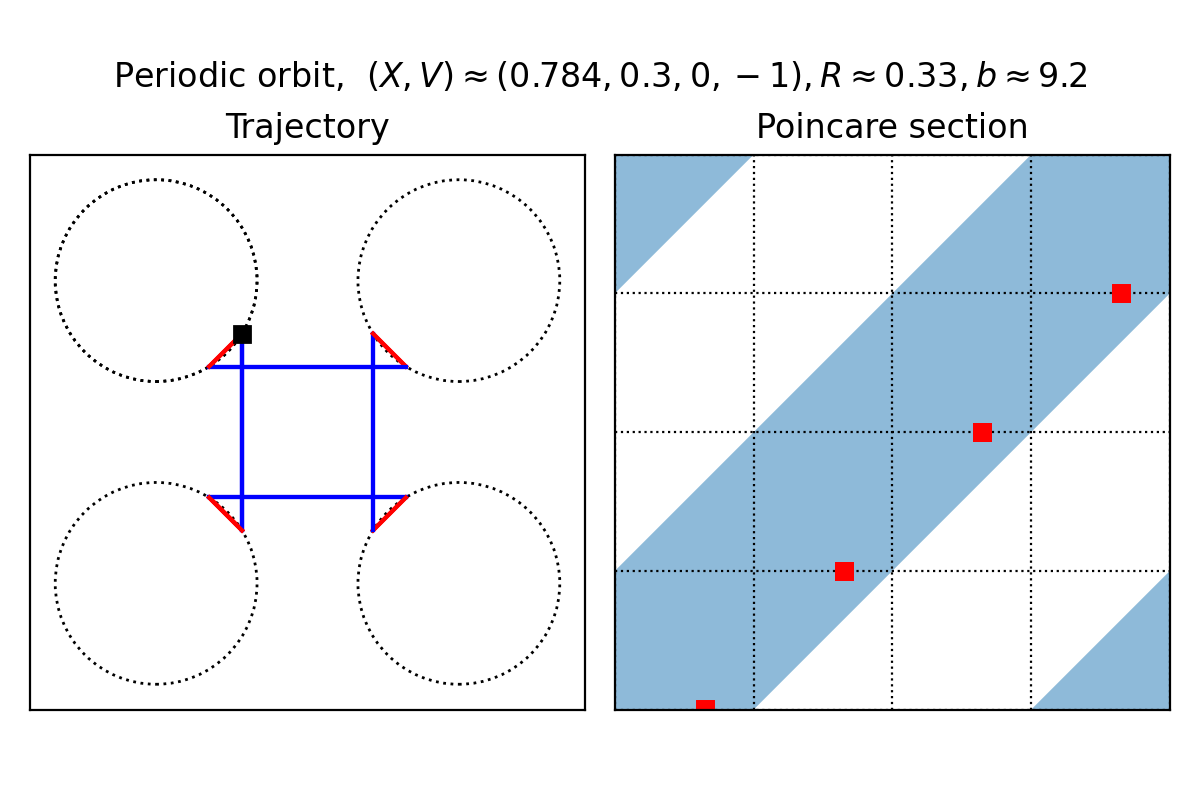
\includegraphics[width=\textwidth, trim={0 1cm 0 0cm}, clip]{unstable_loopy_square_with_poincare.png}
\caption{}
\label{subfig:penandpaperorbits6}
\end{subfigure}
\caption{Unstable trajectories discovered analytically.}
\label{fig:penandpaperorbits}
\end{figure}

The trajectories \cref{subfig:penandpaperorbits1}, \ref{subfig:penandpaperorbits3}, \ref{subfig:penandpaperorbits5}, and \ref{subfig:penandpaperorbits6} are periodic. \Cref{subfig:penandpaperorbits1} and \ref{subfig:penandpaperorbits3} are stable, \hl{we prove this in the python notebook [??]}, and \ref{subfig:penandpaperorbits2} and \ref{subfig:penandpaperorbits4} are given by perturbed initial conditions of each case, respectively. Meanwhile \ref{subfig:penandpaperorbits5}, \ref{subfig:penandpaperorbits6} are unstable, in fact, the plots are given only to 35 iterations due to sensitivity.

\begin{figure}[!th]
\centering
\begin{subfigure}{0.49\textwidth}
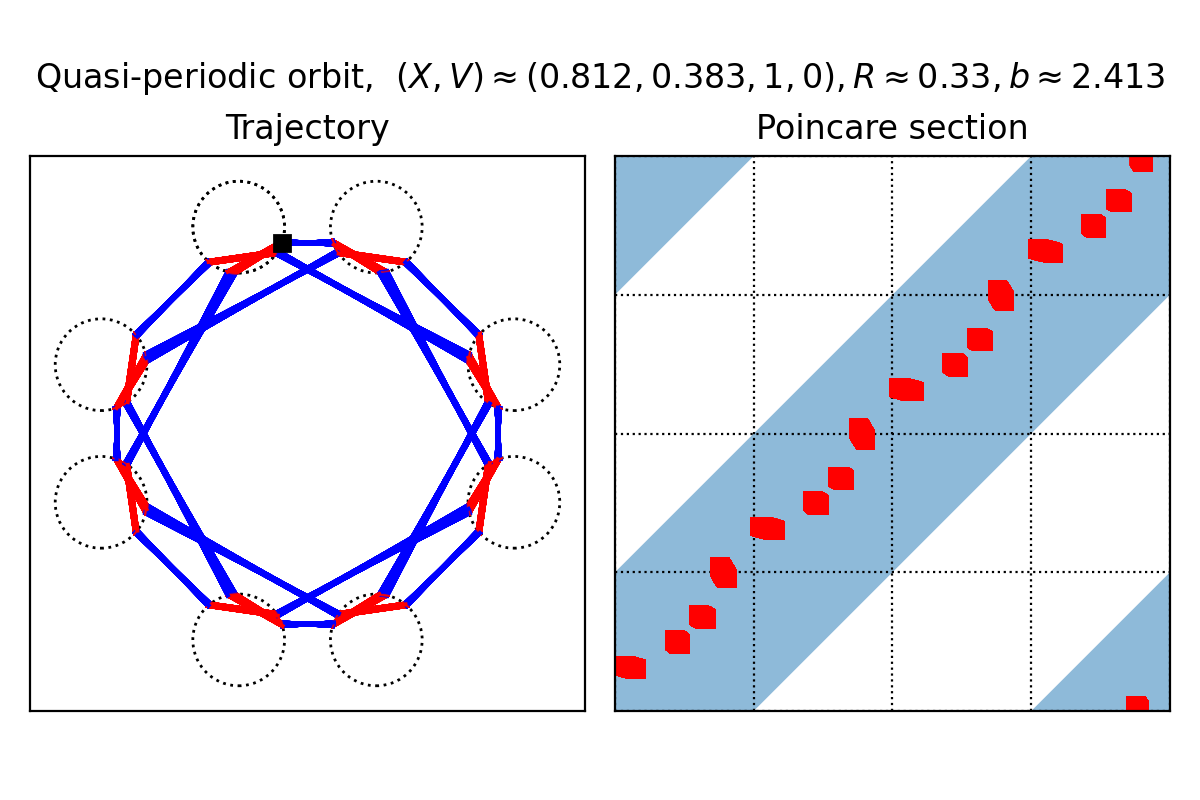
\includegraphics[width=\textwidth, trim={0 1cm 0 0cm}, clip]{star_with_poincare.png}
\caption{}
\label{subfig:star1}
\end{subfigure}
%
\begin{subfigure}{0.49\textwidth}
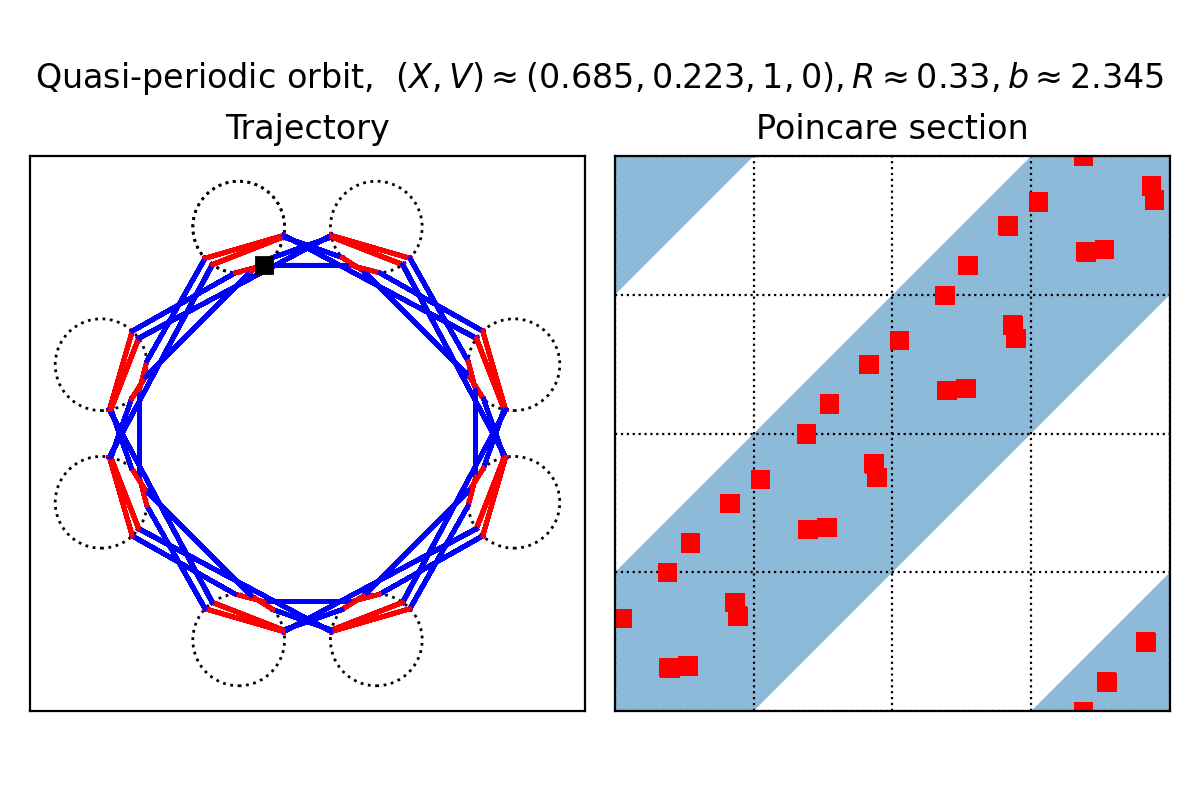
\includegraphics[width=\textwidth, trim={0 1cm 0 0cm}, clip]{doubled_star_with_poincare.png}
\caption{}
\label{subfig:star2}
\end{subfigure}
\caption{First signs of intricate quasi-periodicity.}
\label{fig:stars}
\end{figure}

\Cref{subfig:star1} and \ref{subfig:star2} are interesting, since they have a similar shape. The latter seems to be a ``doubled'' version of the former, and not a perturbation, since even after 2000 iterations the trajectory of \ref{subfig:star2} does not change, e.g., it does not smear like in the case of \ref{subfig:penandpaperorbits2}.

\begin{figure}[!th]
\centering
\begin{subfigure}{0.49\textwidth}
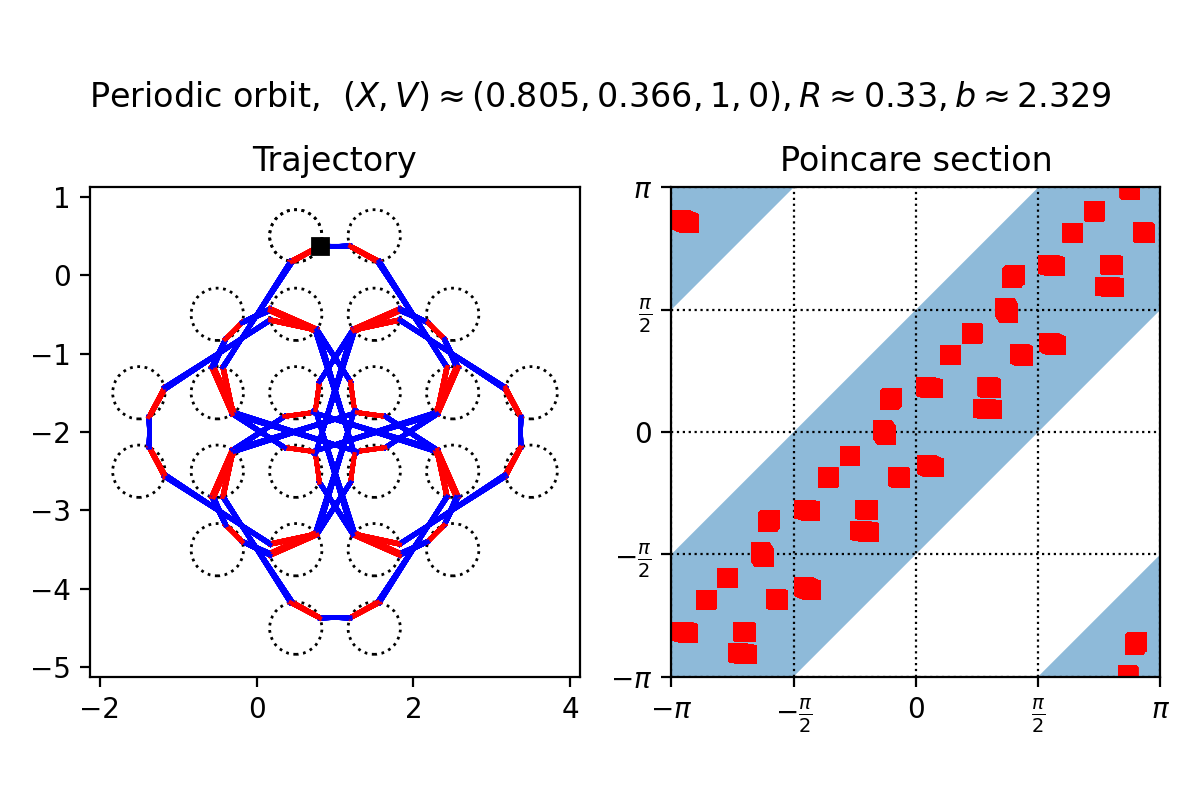
\includegraphics[width=\textwidth, trim={0 1cm 0 0cm}, clip]{sophisticated_with_poincare.png}
\caption{}
\label{subfig:ornamet1}
\end{subfigure}
%
\begin{subfigure}{0.49\textwidth}
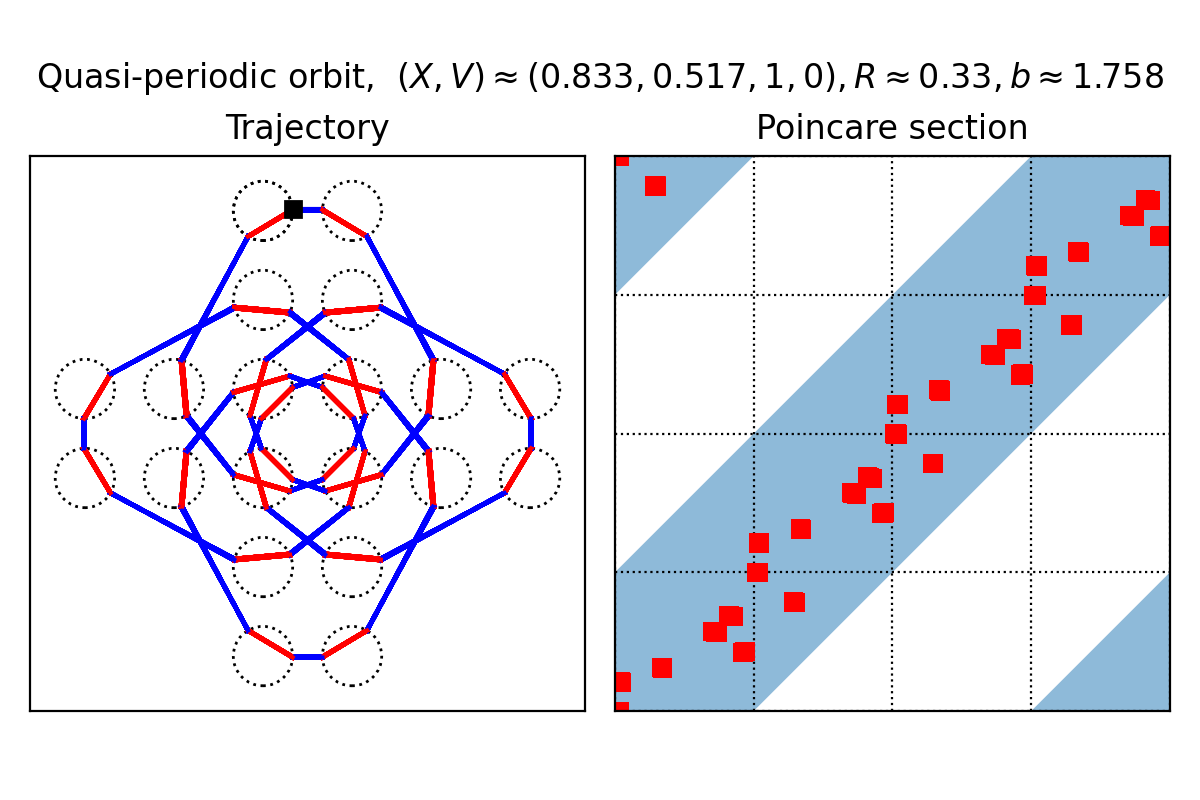
\includegraphics[width=\textwidth, trim={0 1cm 0 0cm}, clip]{distinguished_with_poincare.png}
\caption{}
\label{subfig:ornament2}
\end{subfigure}
\caption{Complex and ornamental quasi-periodic trajectories.}
\label{fig:ornaments}
\end{figure}

\newpage

\Cref{subfig:ornamet1} and \ref{subfig:ornament2} are surprisingly complex patterns, and unlike the rest of the examples, involve the most discs in the plane

\begin{figure}[!th]
\centering
\begin{subfigure}{0.49\textwidth}
\centering
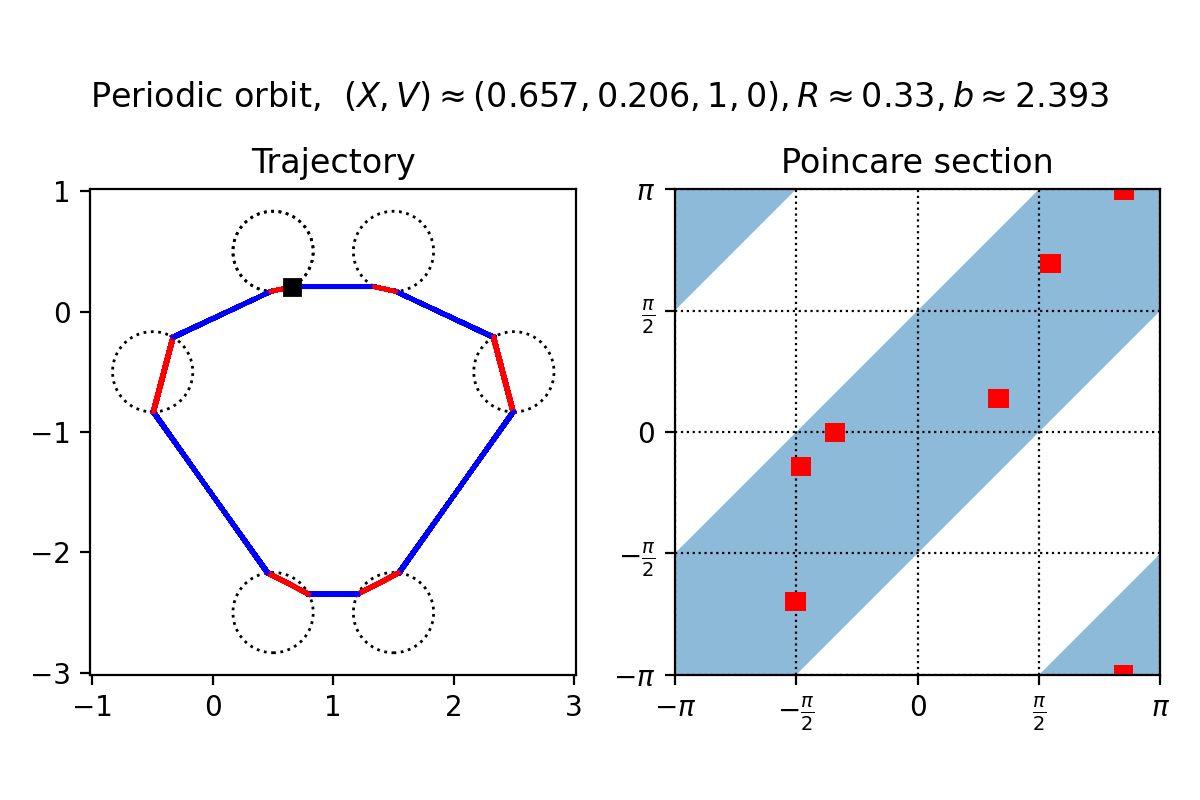
\includegraphics[width=\textwidth, trim={0 1cm 0 0cm}, clip]{lopsided_octagon_with_poincare.png}
\caption{}
\label{subfig:lopsidedhexagon}
\end{subfigure}
%
\begin{subfigure}{0.49\textwidth}
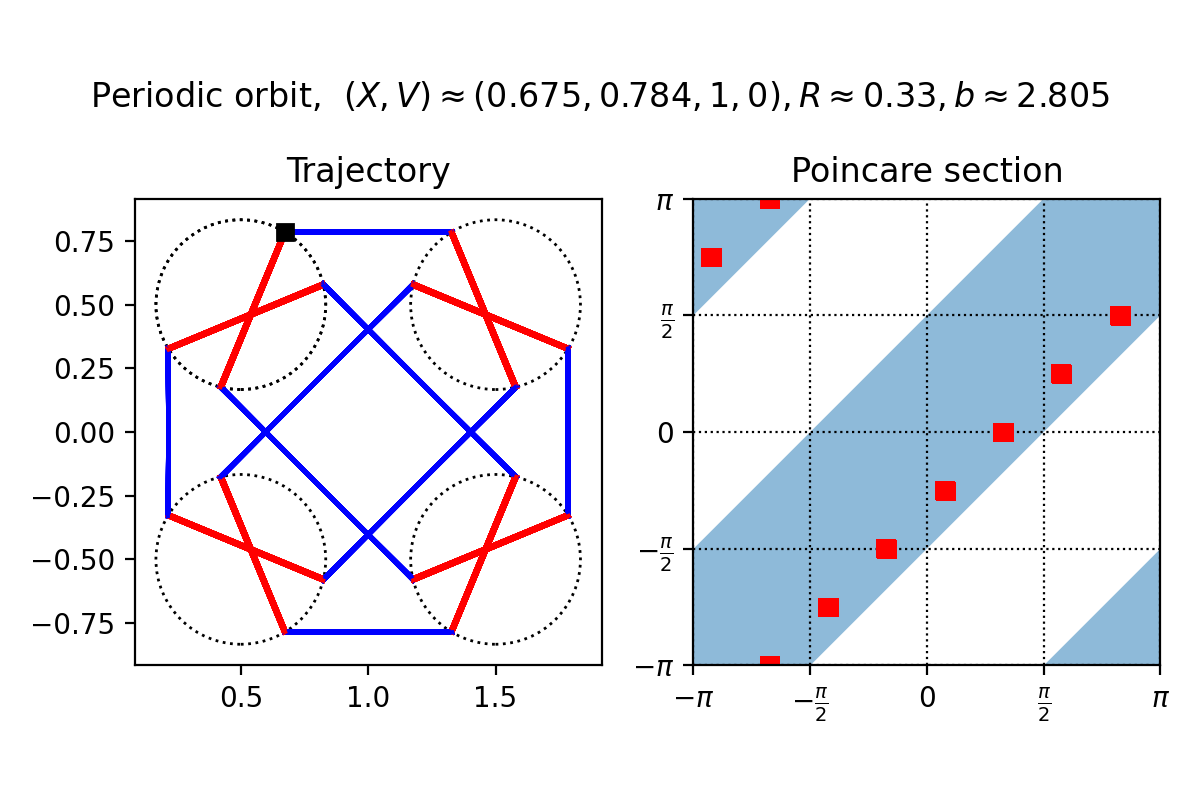
\includegraphics[width=\textwidth, trim={0 1cm 0 0cm}, clip]{strange_square_with_poincare.png}
\caption{}
\label{subfig:strangesquare}
\end{subfigure}
\caption{A symmetry breaking trajectory and an honorable mention.}
\label{fig:honorablementions}
\end{figure}

So far, we have seen trajectories that have square symmetries, the first to break this is \ref{subfig:lopsidedhexagon} with a bottom-heavy hexagon. It would be interesting to see if there are other polygon, for example triangles or pentagons. \Cref{subfig:strangesquare} does not illustrate anything new, we included it because it is aesthetically pleasing.

\begin{figure}[!th]
\centering
\begin{subfigure}{0.49\textwidth}
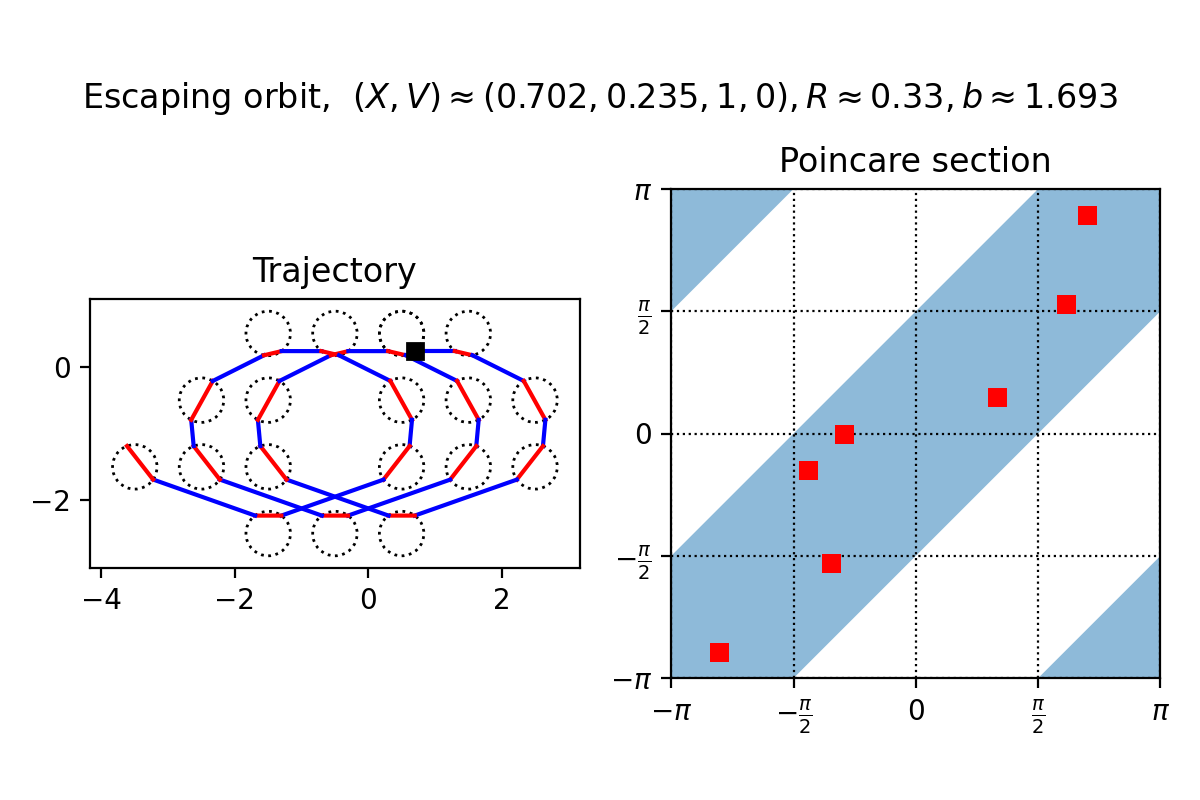
\includegraphics[width=\textwidth, trim={0 1cm 0 0cm}, clip]{walker_with_poincare.png}
\caption{}
\label{subfig:walker1}
\end{subfigure}
%
\begin{subfigure}{0.49\textwidth}
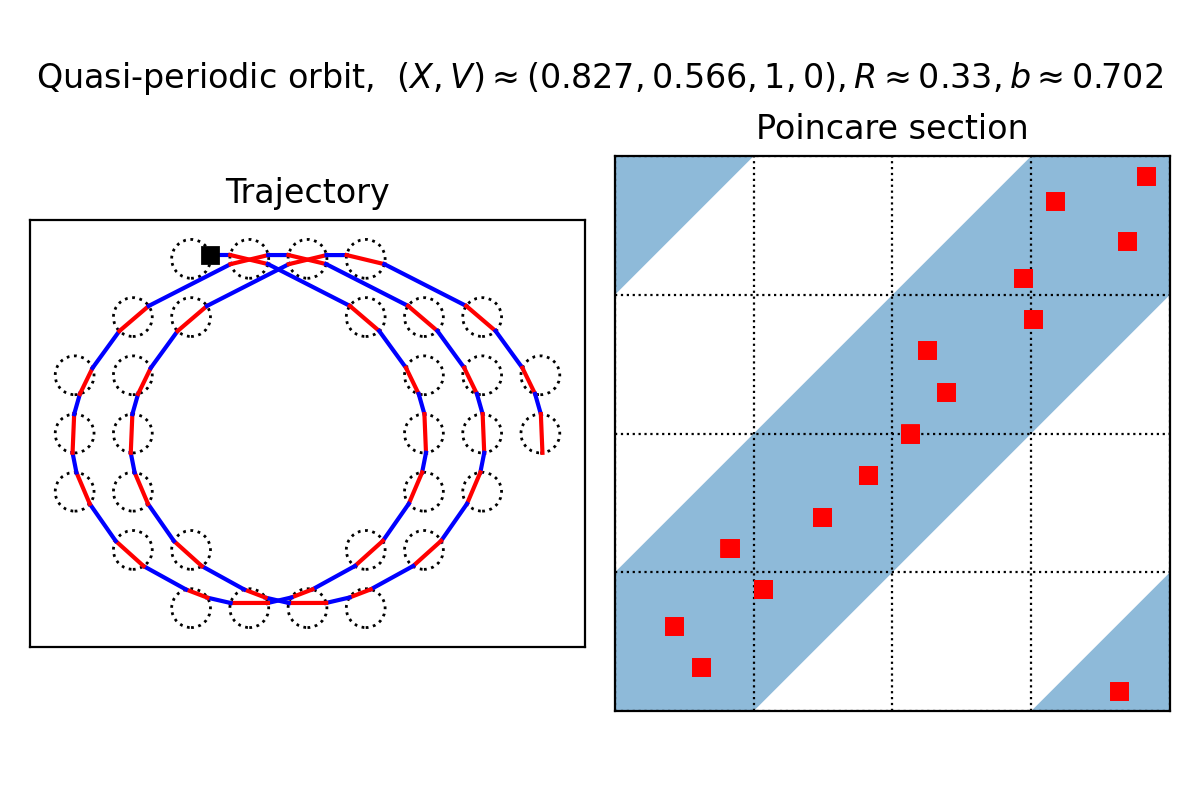
\includegraphics[width=\textwidth, trim={0 1cm 0 0cm}, clip]{big_walker_with_poincare.png}
\caption{}
\label{subfig:walker2}
\end{subfigure}
\caption{Wandering in $\mathbb R^2$, yet quasi-periodic in $\mathbb T$.}
\label{fig:walkers}
\end{figure}

In \cref{subfig:walker1} and \ref{subfig:walker2} we have the first examples of trajectories that wander in the plane but are quasi-periodic in the torus. It seems that these patterns arise in between values of $b$ that produce trajectories as in \cref{fig:bigcircles}, that is, as $b$ decreases, the radii of the circles in the pattern increases, and if, in a specific way, the circle does not close, you can still see repetition.

\begin{figure}[!th]
\centering
\begin{subfigure}{0.49\textwidth}
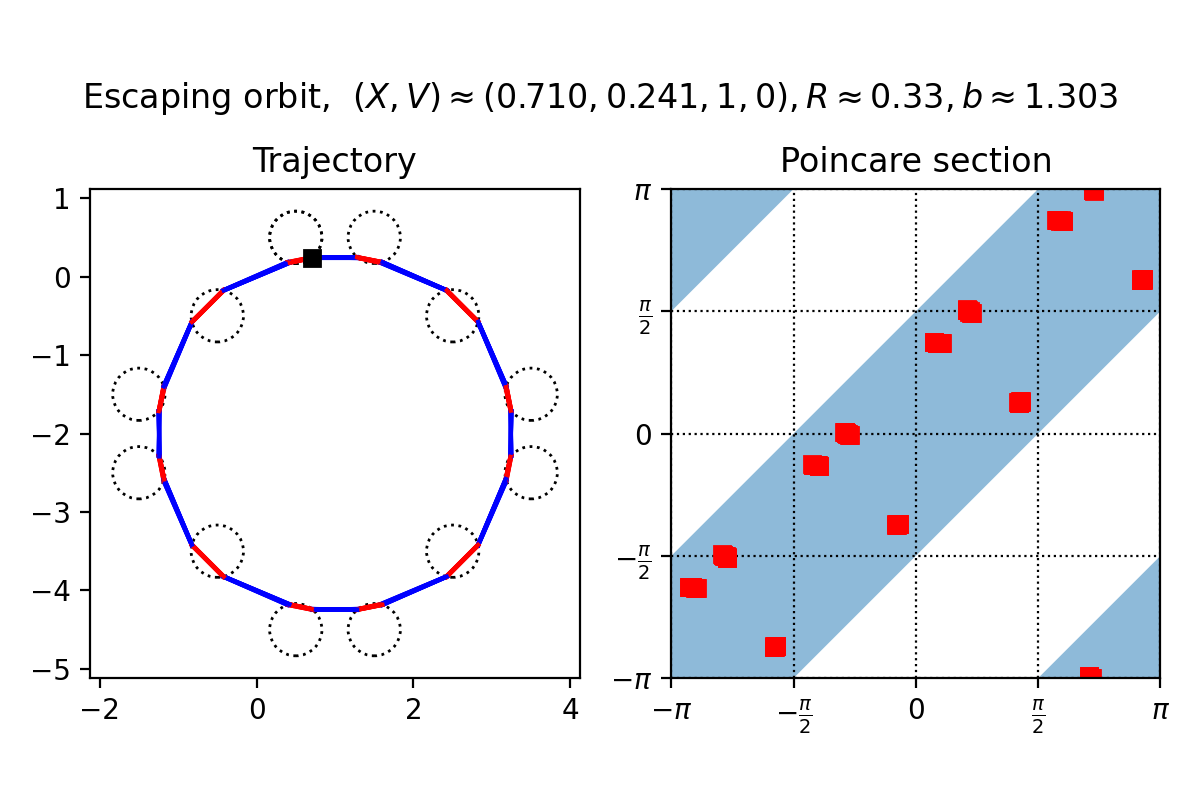
\includegraphics[width=\textwidth, trim={0 1cm 0 0cm}, clip]{12gon_with_poincare.png}
\caption{}
\label{subfig:bigcircle1}
\end{subfigure}
%
\begin{subfigure}{0.49\textwidth}
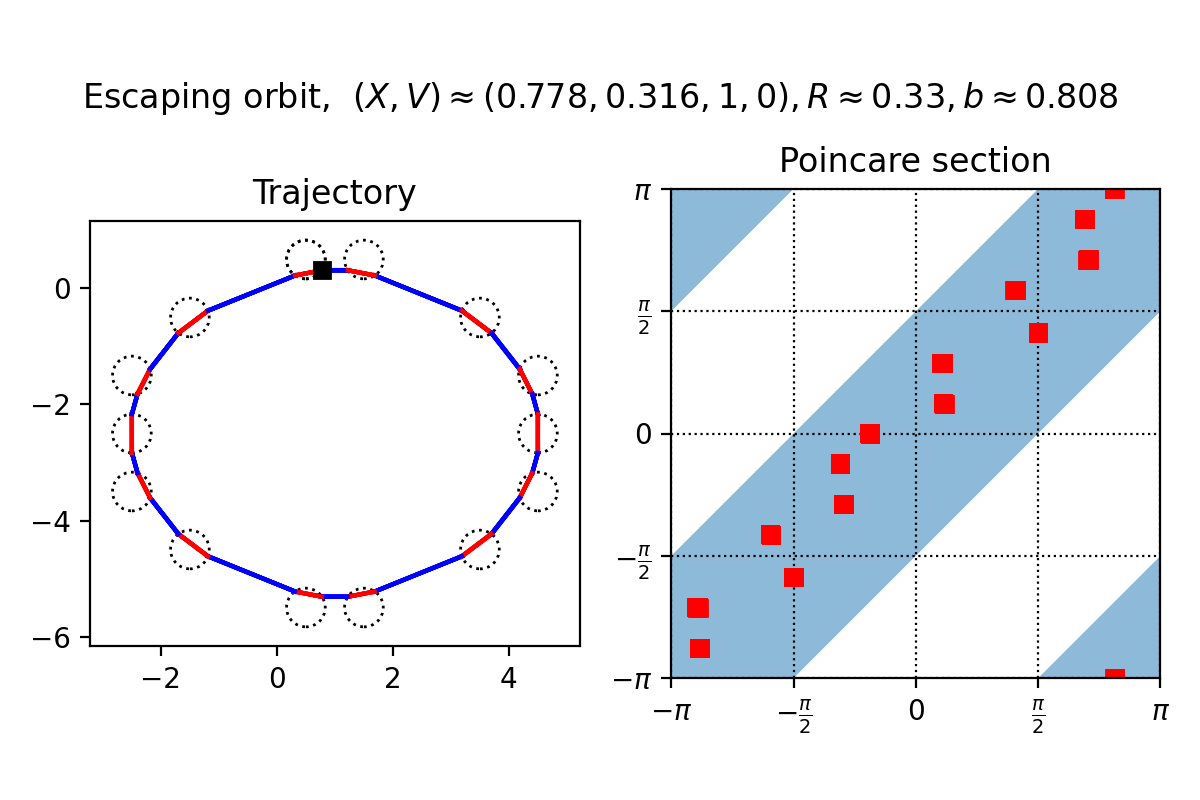
\includegraphics[width=\textwidth, trim={0 1cm 0 0cm}, clip]{egg_with_poincare.png}
\caption{}
\label{subfig:bigcircle2}
\end{subfigure}
%
\begin{subfigure}{0.49\textwidth}
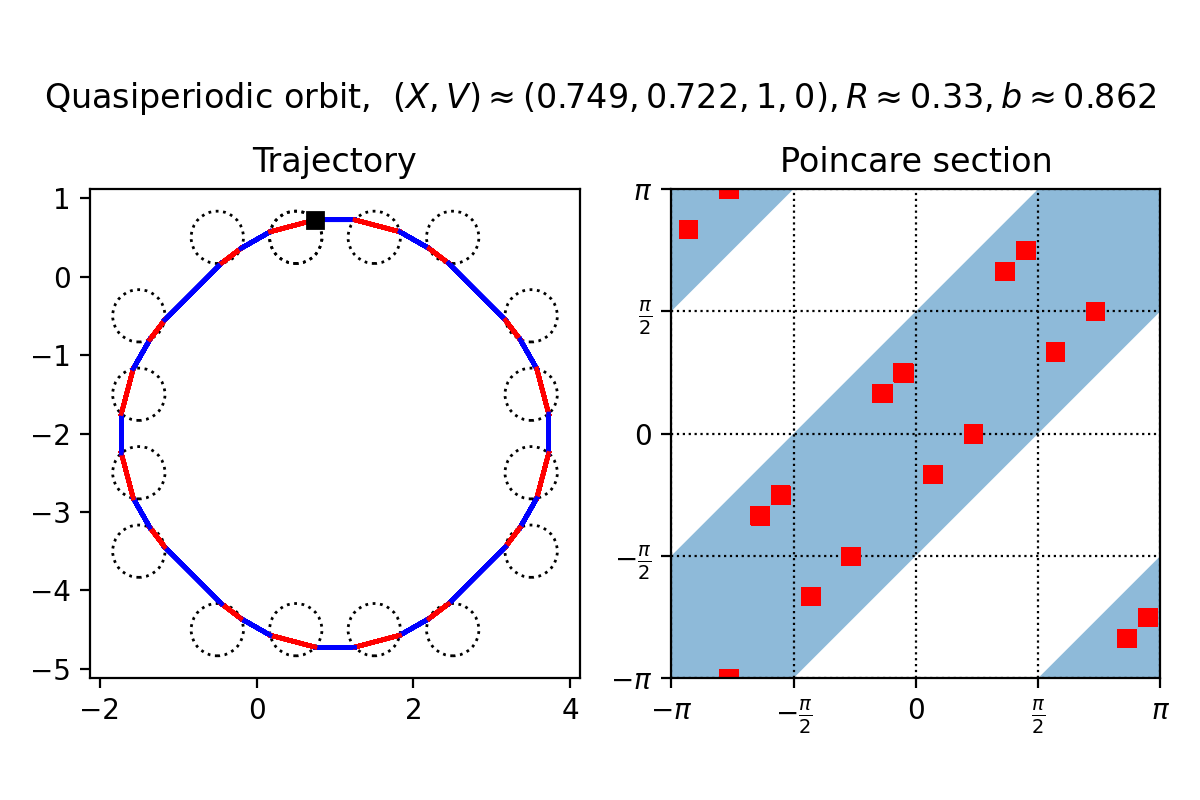
\includegraphics[width=\textwidth, trim={0 1cm 0 0cm}, clip]{big_square_with_poincare.png}
\caption{}
\label{subfig:bigcircle3}
\end{subfigure}
%
\begin{subfigure}{0.49\textwidth}
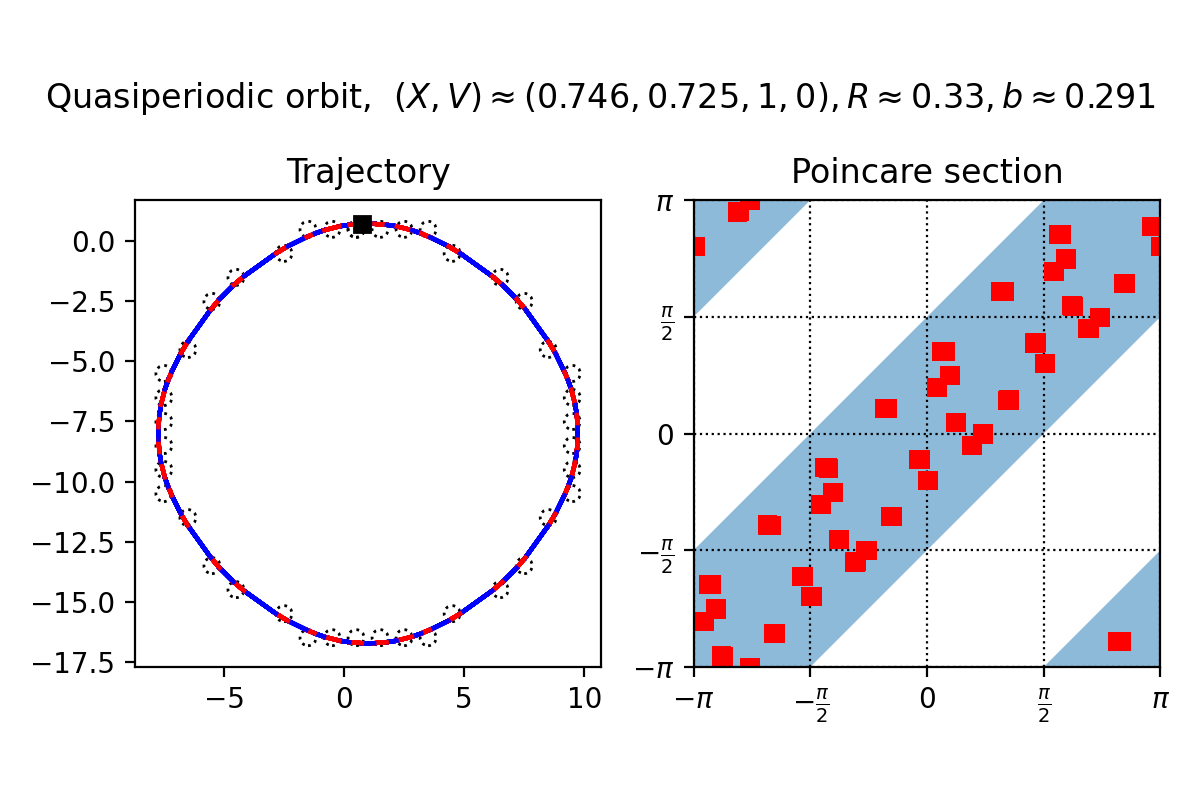
\includegraphics[width=\textwidth, trim={0 1cm 0 0cm}, clip]{big_circle_with_poincare.png}
\caption{}
\label{subfig:bigcircle4}
\end{subfigure}
\caption{Large circular trajectories for small values of $b$.}
\label{fig:bigcircles}
\end{figure}

The last \ref{subfig:bigcircle1} - \ref{subfig:bigcircle4} are examples with values of $b$ relatively small compared to the rest. The lower the value of $b$, the closer the shape resembles a circle, which is in line with what we had seen using KAM. We have not found any intricate patterns for low values of $b$.

We see that in this simple system there is interesting dynamics with varying levels of complexity. It is safe to say that at least some of these would be hard to find by hand, and would be feasible only with some numerics and a measure of complexity for determining good candidates. We now construct the Poincar\'e section $\Sin$ and after that we outline the methods we used to obtain these quasi-periodic trajectories.


\subsection{Constructing a Poincar\'e section}
%\subsection{Constructing a Poincar\'e section}

To construct the Poincar\'e section, we will use well known results about rotations on the torus. Parametrize the torus $\mathbb T$ with angles $\theta,\varphi\in[0,1]$, a particle in free motion on $\mathbb T$ follows the trajectory $r(t)=x_0+vt$ where $x_0\in\mathbb T$ is the initial condition and $v\in\mathbb R^2$ is the velocity. If the angle of $v$ with respect to the axis $\theta$ is rational, then $r(t)$ is periodic, otherwise $r(t)$ is dense in $\mathbb T$.

\begin{lemma}\label{lem:SoutToSin}
The flow of \eqref{eq:magnetichamiltonian} induces a well-defined map $P_\text{oi}:\Sout\to\Sin$.
\end{lemma}
\begin{proof}
Let $(x,v)\in \Sout$, at this point the solution of \eqref{eq:magnetichamiltonian} continues with free motion $r(t)=x+vt$. If the angle of $v$ is rational, then there exists some time $t_2$ at which $r(t_2)=x$, and $(r(t_2),v)\in \Sout$. Since at time $t_2$ the trajectory intersects $\partial S$ transversally, there must exist $t_1<t_2$ such that $(r(t_1),v)\in \Sin$. Since the trajectory intersects $\Sin$ at least once, there must exist a unique $t_0\le t_1$ such that $(r(t_0),v)\in \Sin$.

If instead the angle of $v$ is irrational, consider an open neighborhood $U\subseteq \partial S$ of $x$ such that $U\times\{v\}\subseteq \Sout$. This can be done by taking a sufficiently small interval in $\partial S$ around $x$. Since $r(t)$ is dense in $\mathbb T$, there exists a time $t_1$ such that $r(t_1)\in U$. By the same reasoning as in the previous case, there exists a unique time $t_0$ such that $(r(t_0),v)\in \Sin$.

Define $P_{\text oi}(x,v) = (r(t_0), v)$, which is well-defined.
\end{proof}

\begin{lemma}\label{lem:SinToSout}
The flow of \eqref{eq:magnetichamiltonian} induces a well-defined map $P_\text{io}:\Sin\to\Sout$.
\end{lemma}
\begin{proof}
Let $(x,v)\in \Sin$, under the flow of \eqref{eq:magnetichamiltonian} the trajectory $r(t)$ follows some Larmor circle $C$. We know $x\in C\cap \partial S$, so since $(x,v)$ is transversal to $\partial S$, there must exist a point $x_1\in C\cap\partial S$ with $x_1\neq x$. Hence, also there must exist a time $t_0$ at which the trajectory intersects $\Sout$. Define $P_{\text io}(x,v) = (r(t_0), r'(t_0))$.
\end{proof}

\begin{proof}[Proof of \cref{prop:poincaresurface}]
The map $P_{\text i} = P_{\text oi}\circ P_{\text io}$ is a return map for $\Sin$. Likewise, $P_{\text o} = P_{\text io}\circ P_{\text oi}$ is a return map for $\Sout$.
\end{proof}

The proof of \cref{lem:SoutToSin} does not depend on the shape of the magnetic region. However, \hl{it is not clear what needs to be changed to make } \cref{lem:SinToSout} work for arbitrary regions.

In \cite{Knauf_2017} a similar result is proved for a configuration of finitely many bumps. In that case a different method was used that did not rely on an infinite number of bumps, in ours the reasoning was simplified due to this.


\subsection{Mapping the Poincar\'e section to a Shift space}
To study a discrete dynamical system in terms of symbolic dynamics one usually deduces a Markov partition of the space such that the system in question can be related via a (semi)-conjugacy to a shift-space of finite type. What is obtained is a simpler representation encoding the original dynamics. In the previous section, we successfully reduced the dynamics of \eqref{eq:magnetichamiltonian} to a discrete system on either $\Sin$ or $\Sout$. From now on we focus only on $\Sout$.

A first attempt at establishing symbolic dynamics in our case runs into a few issues. Firstly, the shift map is continous on a shift-space, so provided $\Sout$ has the natural product topology, the map $P_\text{o}:\Sout\to\Sout$ should be continuous as well. Recall, $P_\text{o} = P_\text{io}\circ P_\text{oi}$, the map $P_\text{io}$ can be shown to be continuous, however $P_\text{oi}$ is definitely not continuous. It is not clear a priori whether $P_\text{o}$ is continuous, there could exist values of $b$ which make it so. However, it is reasonable to assume that in general $P_\text{o}$ is discontinuous. So, we should find a different topology on $\Sout$ for this method to work.

Next, it seems constructing a Markov partition is difficult. In the construction, we need to consider the stable and unstable sets of points in $\Sout$ under iteration of $P_\text{o}$, and by definition $P_\text{o}$ must be at least differentiable, which we know it is not. Ignoring this issue, we can look for any reasonable partition that does not have the Markov property. 

A reasonable partition should be finite, this way we can salvage some intuition from the above method. Focusing on the effects of $P_\text{oi}$, we see that, with the right conditions, a trajectory could jump to one of an infinite number of other circles relative to the circle we start from. So, to have a finite partition, some concessions must be made. We could partition in such a way that jumps to a circle past a certain radius are all assigned the same symbol. One could also partition the circle lattice in a checkerboard fashion, yet neither of these approaches seem ``natural''. Hence, given all the resistence, we should consider another approach to symbolic dynamics.

Let $a_0=(\theta_0,\varphi_0)\in\Sout$, and define $a_n=P_\text{o}^n(a_0)$, that is, $a_n$ is the $n$-th iterate of $a_0$. In the plane, each circle of $\Sout$ is associated with a coordinate $\mathbb Z^2+1/2$, then to each $a_n$ we associate the coordinate $s_n$ of the circle which $a_n$ is on. Now, to the sequence of iterates $\{a_n\}_{n\ge 0}$ we associate the sequence of symbols $\{s_{n}-s_{n-1}\}_{n\ge1}\subseteq \mathbb Z^2$. In other words, the symbols encode the relative jumps of the trajectory. Immediately, we notice that the alphabet we picked is countably infinite which we previously asserted was not \textit{reasonable}, however we argue that this choice makes the least assumptions and hence in a sense is natural. Our choice will be further justified once we introduce the Lempel-Ziv complexity of strings.

\subsection{The Lempel-Ziv compression algorithm}
We introduce the Lempel-Ziv complexity (LZC) as described in \cite{LZ76}. LZC operates on finite length sequences of symbols by applying a compression algorithm, the complexity of the original sequence is then quantified by the result of the compression.

We find it easiest to include the code of the implementation. The code is provided by Mediano and Rosas \cite{MedianoRosas2019} and they attribute the implementation to \cite{Kaspar1987EasilyCM} which is a nice use case and provides a good example of the algorithm.

\begin{lstlisting}[language=python]
def LZ76(ss):
    """    
    Input: ss -- array of integers
    Output: c  -- integer
    """
    i, k, l = 0, 1, 1
    c, k_max = 1, 1
    n = len(ss)
    while True:
        if ss[i + k - 1] == ss[l + k - 1]:
            k = k + 1
            if l + k > n:
                c = c + 1
                break
        else:
            if k > k_max:
               k_max = k
            i = i + 1
            if i == l:
                c = c + 1
                l = l + k_max
                if l + 1 > n:
                    break
                else:
                    i = 0
                    k = 1
                    k_max = 1
            else:
                k = 1
    return c
\end{lstlisting}

Loosely, we have two pointers ascending through the list, the left pointer is at index $i+k-1$, and the right pointer is at index $\ell+k-1$, at each iteration the pointers move depending on what symbol they see at their index. If they see the same symbol, the size of the window $k$ is incremented by 1, so both pointers shift, if not then $i$ is incremented by 1, i.e., only the left pointer shifts. As this happens we update the longest window size $k_\text{max}$ that we encounter, this corresponds to the size of the longest word that can be reconstructed starting at index $\ell$ using only the words that appear before $\ell$. Once $i=\ell$, we increment the number of words, the right pointer is pushed forward by $k_\text{max}$, that is, $\ell$ becomes $\ell+k_\text{max}$. The process repeats until the right pointer reaches the end of the list or if the current window size looks past the end of the list.

We provide examples below. The $\cdot$ is used as a word delimiter, the underline indicates the window at the left pointer, and the overline indicates the one at the right pointer. We only show the longest window that was achieved, notice the index of the longest window is not necessarily unique, and the window ends at the first symbol that differs. 
\begin{align*}
01011010001101110010
&\xrightarrow{(1)}
\underline0\cdot\overline{1}011010001101110010\\
&\xrightarrow{(2)}
\underline{0\cdot1\,\cdot\,}\overline{\underline{0}}\overline{11}010001101110010 \\
&\xrightarrow{(3)}
\underline{0\cdot1\cdot01}1\cdot\overline{0100}01101110010 \\
&\xrightarrow{(4)}
0\cdot1\cdot\underline{011\cdot010}0\cdot\overline{011011}10010 \\
&\xrightarrow{(5)}
0\cdot1\cdot011\cdot0\underline{100\cdot0}11011\cdot\overline{1001}0 \\
&\xrightarrow{(6)}
\underline{0\cdot1}\cdot011\cdot0100\cdot011011\cdot1001\cdot\overline{0\text{  }},
\end{align*}
the number of words is 7, so the LZC of this sequence is $7$. Let's consider another example with repetition:
\begin{align*}
01101101101101101101
&\xrightarrow{(1)}
\underline0\cdot\overline{1}101101101101101101\\
&\xrightarrow{(2)}
0\cdot\underline{1\,\cdot\,}\overline{\underline{1}}\overline{0}1101101101101101\\
&\xrightarrow{(3)}
0\cdot\underline{1\cdot10\,\cdot\,}\underline{\overline{11011011011011}}\overline{01\text{  }},
\end{align*}
the number of words is 4, so the LZC is 4. Notice how the two examples have the same number of digits but the one with less repetition has greater complexity. We consider one final example:
\begin{align*}
01010101010101010101
&\xrightarrow{(1)}
\underline{0}\cdot\overline{1}010101010101010101\\
&\xrightarrow{(2)}
\underline{0\cdot1\,\cdot\,}\underline{\overline{01010101010101010}}\overline{1\text{  }},
\end{align*}
and we see the LZ complexity is 3. Notice that even though the last two examples are periodic, one has greater LZC, since the repeating word 011 is longer than 01. So, LZC not only differentiates between periodic and aperiodic sequences, it also distinguishes between periodic sequences of different period.

All examples were with the alphabet $\{0,1\}$ but this can be done with an arbitrary alphabet. It's interesting to note that LZC also supports infinite alphabets. Since we consider finite sequences, there is an upper bound for LZC, namely, the length of the sequence. We have yet to find a drawback in the setup.

The LZC is suited for comparing sequences of the same length. We can see this is the case by comparing $010$ and $010101\dots$, the latter can be made arbitrarily long and the two LZC will be still the same. Yet, this is meaningless, since the LZC of a short sequence will be comparable to its length.

Now, suppose we consider sequences generated by \eqref{eq:magnetichamiltonian} using the procedure as discussed in the previous section. In this case the sequences encode information about trajectories of a dynamical system. We can apply LZC to these sequences to distinguish between periodic and aperiodic trajectories, though, since we use LZC for finite length sequences, we only compare trajectories up to a finite time horizon. Many structures in dynamical systems rely on infinite times, for example, limit cycles, so LZC may or may not detect them. Likewise, there exist systems with trajectories that can stay close to limit cycles for arbitrarily long times before diverging, so LZC could not detect this behavior unless a longer time horizon is chosen. 

In fact, we see this type of behavior in \cref{fig:sensitive_trajectory}: if we took symbols up until the trajectory just jumped out from the 4 bumps, then the LZC would be very low for the length of the sequence, yet clearly the trajectory is not quasi-periodic. Focusing on the trajectories in \cref{fig:weakcomparison}, we see that another issue can arise: the chosen time horizon could be shorter than the period of the (quasi)-periodic trajectory, LZC could label such a trajectory as complex despite the ``macroscopic'' structure that is apparent with the human eye. LZC would also struggle with eventually periodic sequences, if the periodic behavior arrives too late, then the LZC ranks the trajectory complex.

\subsection{Lempel-Ziv varying $b$ and initial conditions}
\begin{figure}[!th]
\centering
\begin{subfigure}[h]{\textwidth}
\centering
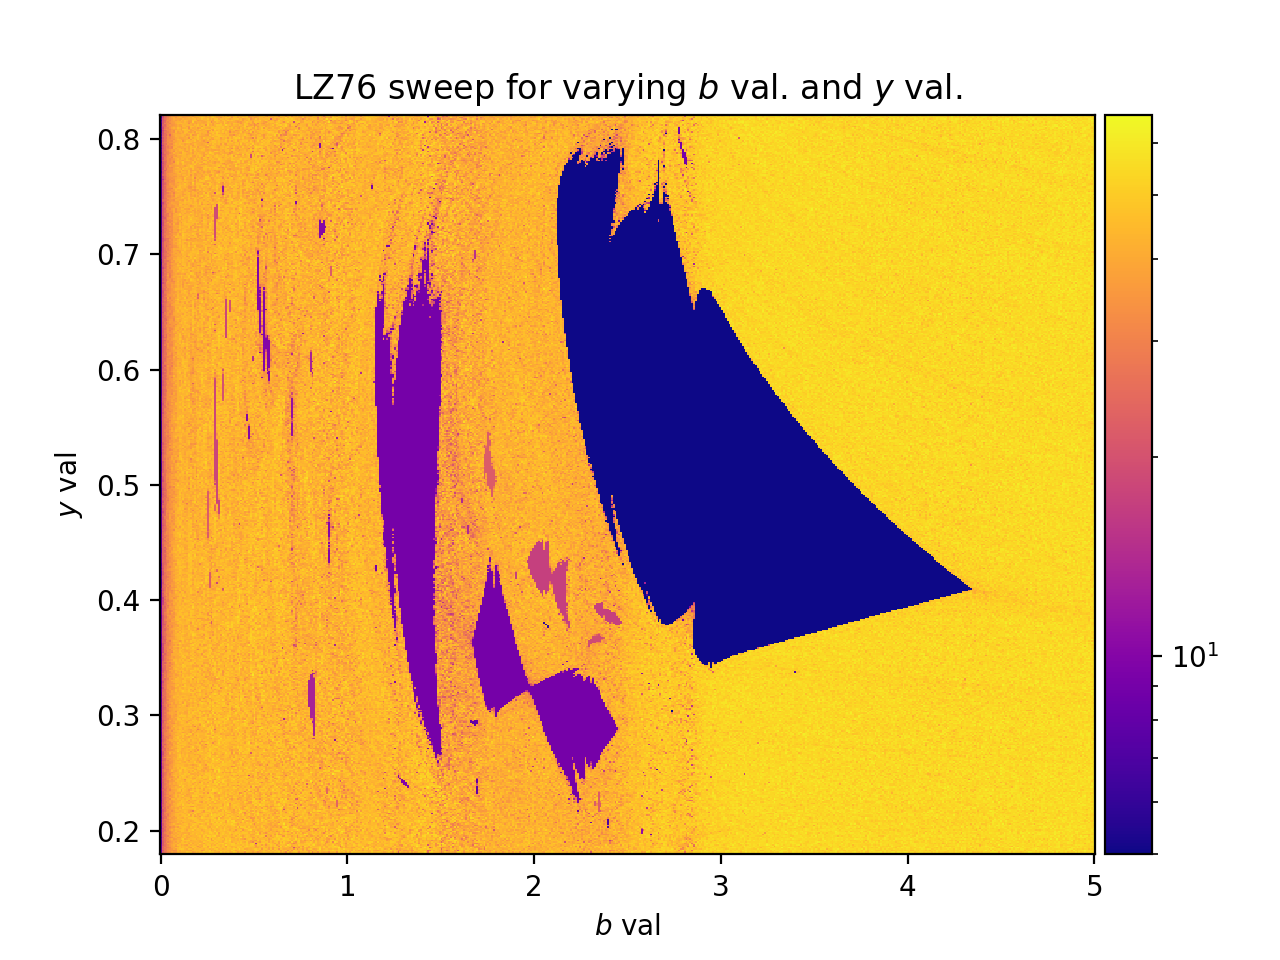
\includegraphics[width=\textwidth, trim={0cm 0cm 0cm 0cm}, clip]{LZ_b_Y_sweep.png}
\caption{}
\label{subfig:LZsweepYandb}
\end{subfigure}
%
\begin{subfigure}[h]{\textwidth}
\centering
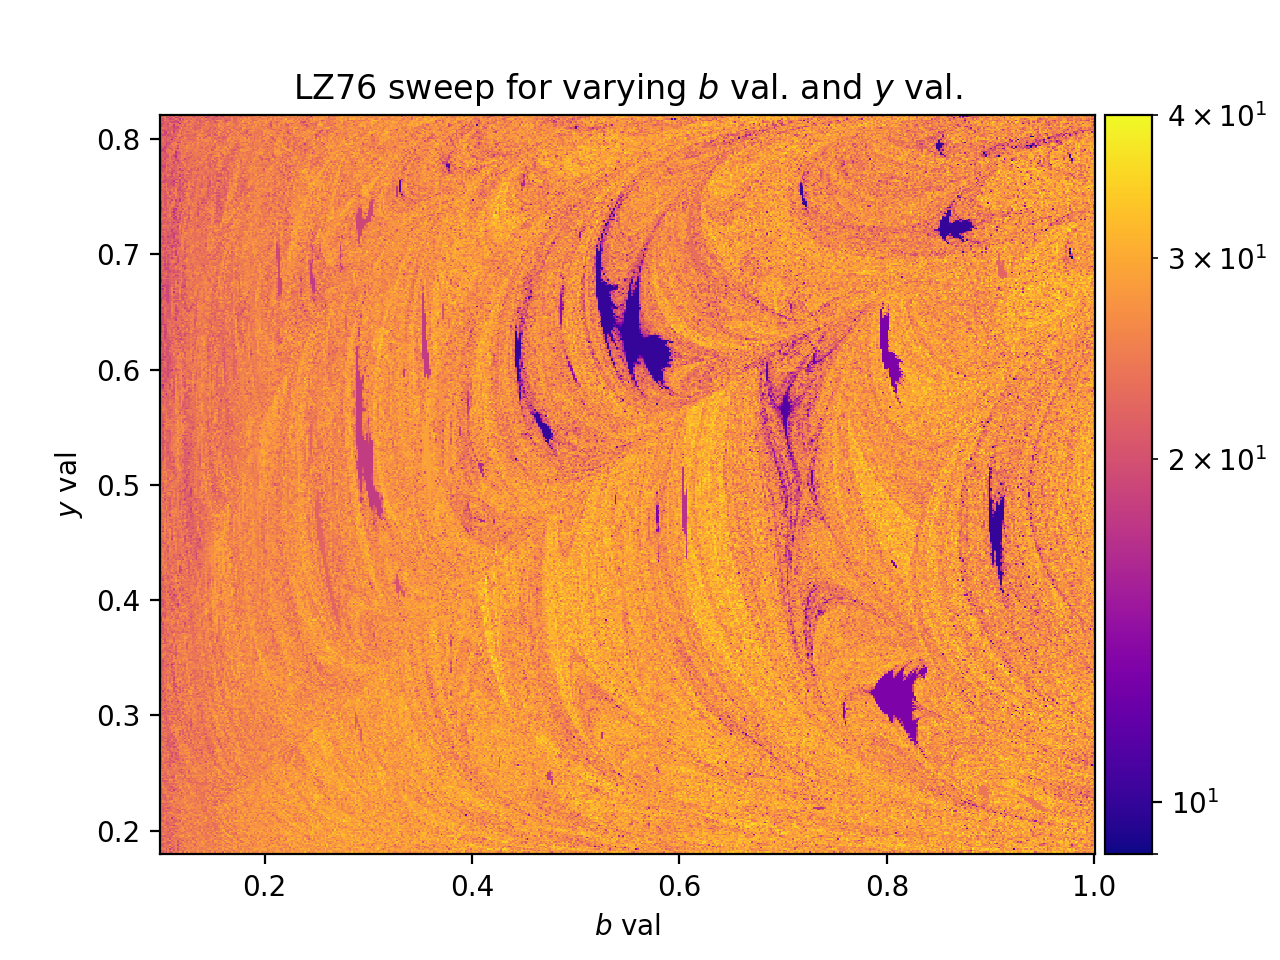
\includegraphics[width=\textwidth, trim={0cm 0cm 0cm 0cm}, clip]{LZ_b_(01_1)_Y_sweep.png}
\caption{placeholder}
\end{subfigure}
\caption{}
\end{figure}

\subsection{Lempel-Ziv Poincar\'e sections for fixed $b$}
A commonn method of analyzing dynamical systems is plotting a trajectory's return to a Poincar\'e section. In some cases one can also use it to prove the existence of a limit cycle or chaotic behavior. When it comes to visualization, one can only plot a handful of different trajectories in a Poincar\'e section before the image becomes too busy and illegible, so we see the details of a selection of trajectories and not the full picture.

We propose to apply a similar procedure for Poincar\'e sections as in the previous section: fix a value for $b$, and sample initial conditions on the Poincar\'e section, and compute LZC for each. If the resolution and depth of iteration is high enough. In such a way, we achieve a general picture of the dynamics.

Recall, the Poincar\'e section is parametrized by two angles $\theta$ and $\varphi$, the former is for the position, and the latter for the direction of the velocity. We fixed the speed to be 1. We only consider $\theta\in[-\pi/4,\pi/4]$, that is, only the right ``side'' of the circle $\Sout$. We do not lose information doing this, since system \cref{eq:magnetichamiltonian} has 4-fold rotational symmetry due to the lattice arrangement of the magnetic discs. The lattice is invariant under all square symmetries, but since the magnetic field always turns trajectories to the right, we cannot use reflections to further shrink the window to plot.

\begin{figure}[!th]
\centering
\begin{subfigure}[h]{0.49\textwidth}
\centering
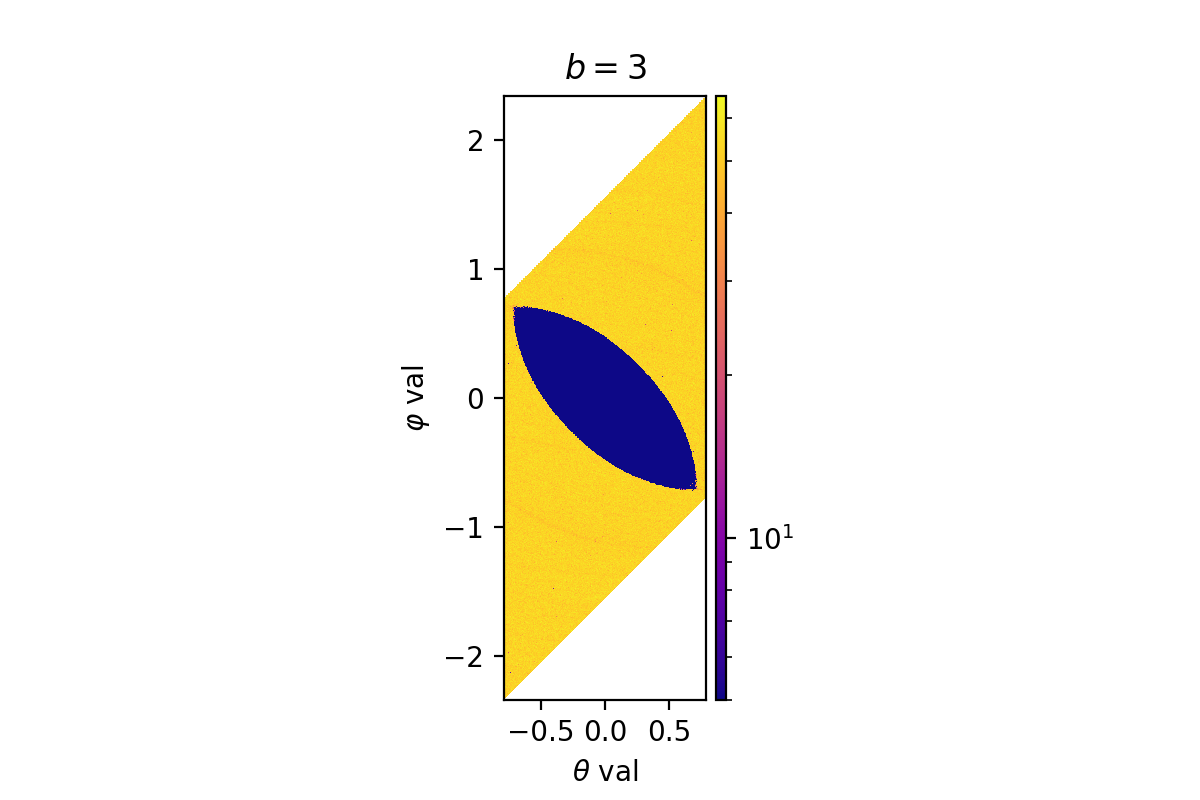
\includegraphics[width=\textwidth, trim={5cm 0cm 4cm 0cm}, clip]{LZ_th_ph_b_3_sweep.png}
\caption{}
\label{subfig:LZpoincaresectionb3}
\end{subfigure}
%
\begin{subfigure}[h]{0.49\textwidth}
\centering
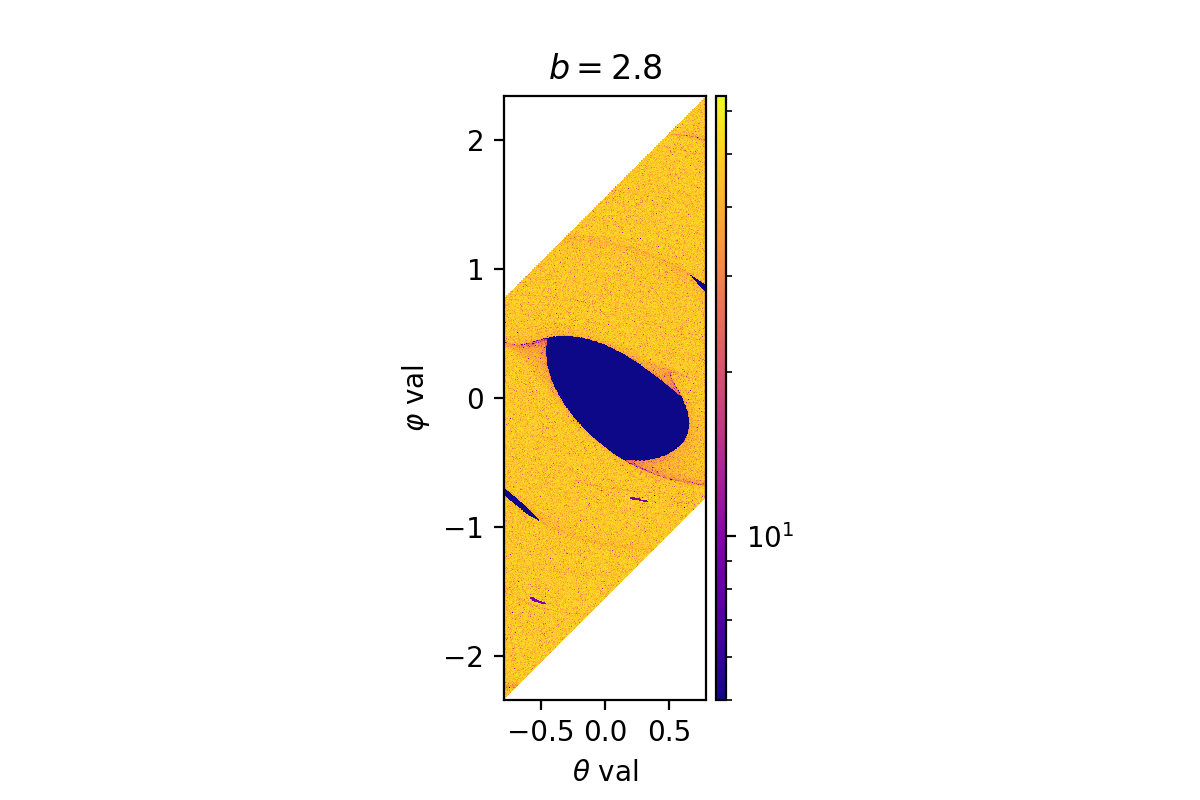
\includegraphics[width=\textwidth, trim={5cm 0cm 4cm 0cm}, clip]{LZ_th_ph_b_2.8_sweep.png}
\caption{}
\label{subfig:LZpoincaresectionb2.8}
\end{subfigure}
\caption{LZC plot of a few Poincar\'e sections}
\label{fig:LZpoincare1}
\end{figure}

In \cref{subfig:LZpoincaresectionb3}, we again focus on $b=3$, which has the periodic trajectory \cref{subfig:penandpaperorbits1}. The dynamics appears to be simple, there is a large region of quasi-periodic trajectories around $(\theta,\varphi)=(0,0)$, and the rest is uniformly high LZC. In \cref{subfig:LZpoincaresectionb2.8}, we perturb $b=2.8$, the stable region from \ref{subfig:LZpoincaresectionb3} changed shape, it is smaller, and there are now more noticeable artifacts along the boundary. Besides that, we see new stable regions: one larger, and two small. The two small ones likely belong to the same quasi-periodic trajectory, while the larger region belongs to its own. Looking back at \cref{subfig:strangesquare}, since there we had $b=2.805$, we see indicated a periodic trajectory along the bottom edge of the Poincar\'e section. Here, we expect a similar trajectory, perhaps slightly perturbed. It's interesting to note that in \cref{subfig:LZpoincaresectionb3} we see faint streaks in the same spots where there are stable regions in \cref{subfig:LZpoincaresectionb2.8}. We conjecture that the patterns and streaks in the noise suggest a nearby bifurcation.

\begin{figure}[!th]
\centering
\begin{subfigure}[h]{0.49\textwidth}
\centering
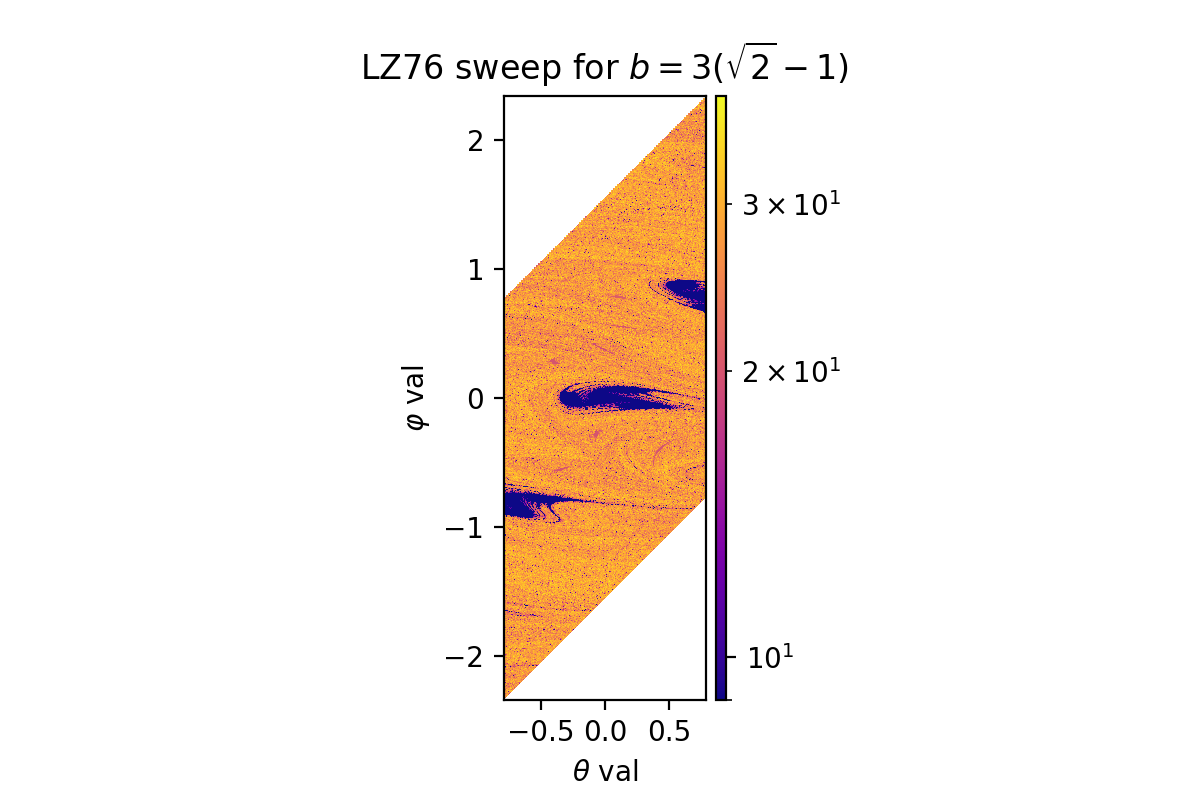
\includegraphics[width=\textwidth, trim={5cm 0cm 4cm 0cm}, clip]{LZ_th_ph_b_3sqrt2-1_sweep.png}
\caption{}
\label{subfig:LZpoincaresectionb1242}
\end{subfigure}
%
\begin{subfigure}[h]{0.49\textwidth}
\centering
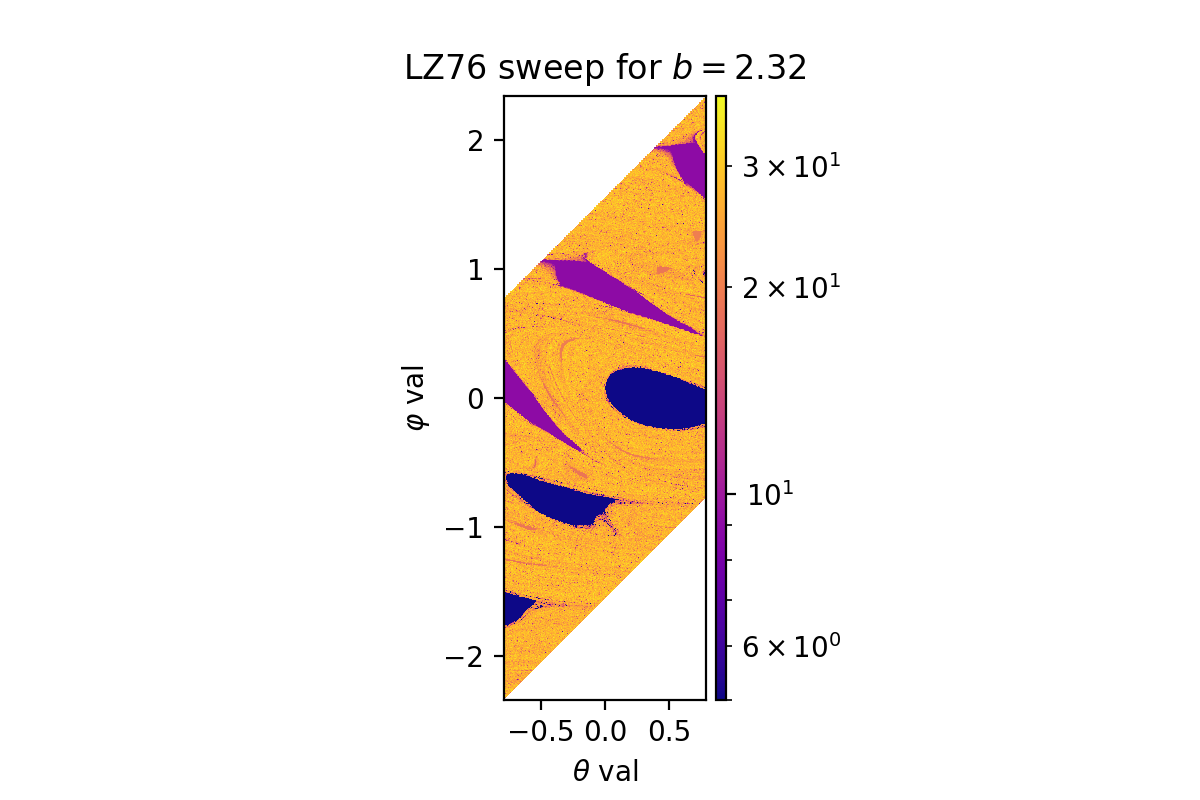
\includegraphics[width=\textwidth, trim={5cm 0cm 4cm 0cm}, clip]{LZ_th_ph_b_2_32_sweep.png}
\caption{}
\label{subfig:LZpoincaresectionb232}
\end{subfigure}
\caption{Another  LZC plot of a few Poincar\'e sections}
\label{fig:LZpoincare2}
\end{figure}
In \cref{subfig:LZpoincaresectionb1242} we plot the same data except $b\approx3(\sqrt2-1)$, corresponding to \cref{subfig:penandpaperorbits3}. The size of the blue regions is about the same, so there should relate to the same quasi-periodic orbit. What's different in this case is the pronounced teardrop with fractal-like structure. If we were to iterate deeper, it looks like the fractal branches would connect to make 4 disjoint blue blobs. Around the main big region, we see smaller red specks, suggesting another quasi-periodic trajectory that we didn't expect before.

In \cref{subfig:LZpoincaresectionb232}, $b=2.32$, the kind of quasi-periodicity here should be similar to \ref{subfig:lopsidedhexagon}, \ref{subfig:ornamet1}, and \ref{subfig:star2}. It's plausible there are 3 different quasi-periodic regions here, since you can separate the blobs easily into three sets: blue along the bottom, purple along the top, and small red in between.



\newpage

\section{Levy Flights}

\newpage

\section{Conclusion}
\subsection{Further questions}

\begin{table}[!ht]
\centering
\renewcommand\arraystretch{2}
\begin{tabular}{>{\raggedright}p{0.2\linewidth}
				>{\raggedright}p{0.2\linewidth}
				>{\raggedright}p{0.2\linewidth}
				>{\raggedright\arraybackslash}p{0.2\linewidth}
                }
\toprule
 & $b\ll1$ & $b\approx1$ & $b\gg1$ \\
\midrule
Uniform perturbation in a disk 
  & Circle Maps 
  & test cases (difficult in general)
  & Perturbation of Sinai Billiards (maybe) \\
Arbitrary perturbations
  & Usual KAM
  & use paper by Donnay-Liverani
  & Hard?\\
\bottomrule
\end{tabular}
\caption{What it is that we want to do}
\label{tab:outline}
\end{table}

\newpage

\bibliographystyle{alpha}
\bibliography{references.bib}


\end{document}